\chapter{Expertenbefragung zur Verwaltungsentwicklung}
Nach der Auswertung der Literatur zur Problematik der Verwaltungsmodernisierung im Westbalkan und der Herausarbeitung des Einflusses, den die EU-Erweiterung auf die Verwaltungsentwicklung hat, sowie der detaillierten Betrachtung von historischen Legacies, die möglicherweise bis in die heutige Zeit nachwirken, werden nun anhand von Experteninterviews die offenen Fragen zur weiteren Entwicklung betrachtet. Dieser Einblick in die Praxis der Verwaltungsmodernisierung im Erweiterungsprozess liefert zusätzliche Erkenntnisse zur Beantwortung der Untersuchungsfragen der vorliegenden Arbeit.\par
Die vorrangig klärungsbedürftig erscheinenden Fragen wurden zu einem Interviewleitfaden gebündelt, der auf der Grundlage der vorherigen Literaturauswertung erstellt wurde. Der Leitfaden enthält die Fragen, die beantwortet werden sollen, und stellt eine Art Richtschnur für den Interviewer dar. Der Interviewleitfaden soll ein allzu weites thematisches „Abdriften“ während des Interviews vermeiden und dennoch Flexibilität in der Gesprächsführung ermöglichen. Aufgrund dieser Spielräume bei der konkreten Gestaltung des Interviews, bei dem gleichzeitigen Versuch alle zu behandelnden Themen unterzubringen, werden solche Interviews gelegentlich auch als „teilstandardisierte Interviews“ bezeichnet (vgl. \cite{flick10}: 223).\par
Die Klassifizierung von Interviews ist dem folgenden Schema zu entnehmen, wobei das halbstandardisierte Interview im Wesentlichen dem teilstandardisierten Interview entspricht:

\begin{table}[H]
\caption[Interviewtypen in der qualitativen Sozialforschung]{Interviewtypen in der qualitativen Sozialforschung}
\center
\scriptsize{
\begin{tabular}{|L{40mm}|L{40mm}|L{40mm}|}\hline
&Fragewortlaut und -reihenfolge&Antwortmöglichkeiten\\\hline
Standardisiertes Interview&
Vorgegeben&
Vorgegeben\\\hline
Halbstandardisiertes Interview&
Vorgegeben&
Nicht vorgegeben\\\hline
Nichtstandardisiertes Interview&
Nicht vorgegeben (nur Thema)&
Nicht vorgegeben\\\hline
\end{tabular}\\
\vspace{0,5cm}
Quelle: \cite{glalau10}: 41. 
}
\end{table}
 
Diese Tabelle stellt die unterschiedlichen Herangehensweisen zur Interview-Durchführung im Überblick dar. Das für die vorliegende Untersuchung gewählte Verfahren der halbstandardisierten Durchführung arbeitet mit vorgegebenen Fragen in einer von der Interviewerin vorher festgelegten Reihenfolge. Die Antwortmöglichkeiten sind allerdings nicht vorgegeben und der Interviewte hat viel Raum, die persönliche Sichtweise und Einschätzung einfließen zu lassen. Es kann daher auch zu Überlappungen in der Beantwortung der Fragen durch den Interviewten kommen, die in der Auswertung und thematischen Zuordnung der Antworten zu berücksichtigen sind.
\section{Themen der Expertenbefragung} 
Thematisch wird an die zentralen Untersuchungsfragen sowie an die bisherigen Auswertungsergebnisse angeknüpft. Mit den Experteninterviews wird eine weitere Sichtweise in die Untersuchungen einbezogen, mit der die bisherigen Ergebnisse im Sinne des methodischen Konzepts der Triangulation ergänzt, unterstützt, aber auch relativiert werden können.\par
Für die Interviews ist zunächst ein Überblick sinnvoll über die Einschätzungen der Interviewpartner zur Bedeutung von Verwaltungsmodernisierung im Zusammenhang mit der Erweiterungsdebatte. Wie schon erörtert wurde, ist die Verwaltungsmodernisierung kein eigenständiges Kapitel des Acquis. Dennoch ist eine leistungsfähige öffentliche Verwaltung notwendig, um die einzelnen Aufgaben bei der Übernahme des Acquis vor dem Beitritt zur EU zu organisieren und durchzuführen. Auch die Verwaltung der EU-Förderpro"-gramme vor dem Beitritt erfordert einen öffentlichen Sektor, der bestimmten Mindeststandards entspricht.\par
Hierzu wurde folgende Frage gestellt:\par
\begin{itemize}[label={}]
\item \ul{Public Administration Reform is not a separate chapter in the Acquis. Should it be a separate chapter?}
\end{itemize}
Neben der Bedeutung der öffentlichen Verwaltung im Beitrittsprozess sind die hemmenden und die fördernden Faktoren für die Verwaltungsentwicklung auf dem Westbalkan von Interesse. Hierzu wurde folgende Frage gestellt:
\begin{itemize}[label={}]
\item \ul{In your opinion, are there obstacles to PAR in Albania, Macedonia and Montenegro? And what would be necessary for successful PAR in Albania, Macedonia and Montenegro?}
\end{itemize}
Speziell sind in diesem Zusammenhang auch die Einschätzungen der Experten von Interesse zur Bedeutung der nachwirkenden historischen Verfahrensweisen sowie zur Übertragbarkeit von Erfahrungen aus früheren Beitrittswellen. Hierzu wurden folgende Fragen gestellt:
\begin{itemize}[label={}]
\item \ul{The literature on enlargement sometimes argues with the legacy theory, in particular regarding the last wave of enlargement. Meaning that structures of previous regime set-ups have an influence on the present development of Public Administration Reform. What is your view on this issue regarding Albania, Macedonia and Montenegro?}
\item \ul{Do you perceive differences in the EU approach compared with the experience with PAR during the last wave of enlargement?}
\end{itemize}
Weitere Fragen zur Verwaltungsmodernisierung betreffen die aktuellen (Finanz-)Pro"-gramme der EU. Die Förderinstrumente, die im Rahmen der Erweiterungsstrategie zur Verfügung stehen, sind entwickelt und weiterentwickelt worden, um die (potenziellen) Kandidatenländer bei der Übernahme des Acquis communautaire zu unterstützen. Fraglich ist, ob diese aus Sicht der Experten dem Bedarf gerecht werden. Hierzu wurden folgende Fragen gestellt:
\begin{itemize}[label={}]
\item \ul{Which topics/areas are presently dealt with as a priority by the EU regarding Public Administration Reform in Albania, Macedonia and Montenegro? What are the developments you see there?}
\item \ul{Do you think the EU approach regarding Public Administration Reform in Albania, Macedonia and Montenegro is adequate? Or should other aspects be included from your point of view?}
\item \ul{How do you assess the EU-Instruments to promote Public Administration Reform in Albania/Macedonia and Montenegro as regards quantity and effectiveness:
Differentiate per country, if possible}
\begin{itemize}
\item CARDS (phased out)
\item Twinning
\item Twinning light
\item TAIEX
\item IPA
\end{itemize}
\item \ul{Are these programmes well designed for the needs of PAR in Albania/Macedonia and Montenegro or do you perceive a need for adjustment in any of them? (Content or technical)}
\end{itemize}
Das Thema Verwaltungsmodernisierung wird von verschiedenen Abteilungen der EU-Kommission bearbeitet. Ihre wesentlichen Aufgaben sind die jährliche Berichterstattung und die Umsetzung von Projekten zur Verwaltungsmodernisierung in den Zielländern. In den Untersuchungsländern selbst sind die Zuständigkeiten für das Thema Verwaltungsmodernisierung ebenfalls unterschiedlich ausgestaltet. Hierzu wurden folgende Fragen an die Experten gestellt:
\begin{itemize}[label={}]
\item \ul{How do you assess the cooperation within the EU Commission regarding Public Administration reform in Albania, Macedonia and Montenegro with the different Units, DG Enlargement, country desks, special PAR Unit and DG Admin?}
\item \ul{Who is responsible for co-ordinating the PAR activities of all the different donors in Albania, Macedonia and Montenegro and what is happening in this respect at the moment? }
\end{itemize}

\subsection{Auswahl der befragten Experten}
Den ausgewählten Themen entsprechend wurden die zu befragenden Experten ausgewählt. „Als Experten könnte man diejenigen Personen bezeichnen, die in Hinblick auf einen interessierenden Sachverhalt als ‚Sachverständige’ in besonderer Weise kompetent sind“ (\cite{deeke}: 7). Bei Experteninterviews interessiert der Befragte weniger in seinem biographischen Zusammenhang, sondern mehr in seiner Eigenschaft als Experte in einem bestimmten Handlungsfeld. Er wird auch nicht als Einzelfall, sondern als Repräsentant einer Gruppe betrachtet (vgl. \cite{flick10}: 214). Es soll im Rahmen der empirischen Generalisierung Repräsentatives, aber auch Unerwartetes herausgearbeitet werden. Ziel ist es, das „überindividuell Gemeinsame herauszuarbeiten, Aussagen über Relevanzstrukturen, Wirklichkeitskonstruktionen, Interpretationen und Deutungsmuster zu treffen“ (\cite{meuser}: 80).\par
Da es sich um drei verschiedene Untersuchungsländer handelt, ist es erforderlich, aus jedem Staat Experten einzubeziehen. Es wurden pro Untersuchungsland jeweils ein Vertreter der Regierung bzw. der Verwaltung und ein Vertreter einer NGO befragt. Alle Interviewten hatten im sich im Rahmen ihrer beruflichen Tätigkeit intensiv mit dem Thema öffentliche Verwaltung und EU-Erweiterung in dem jeweiligen Land beschäftigt. Die NGO-Vertreter wurden einbezogen in der Annahme, dass sich aus der Sicht von Vertretern der Zivilgesellschaft andere Sichtweisen und andere Einschätzungen ergeben als bei den befragten Regierungs- und Verwaltungsvertretern. Somit wurde versucht eine größere Bandbreite an nationalen Einschätzungen zu erreichen. Die Auswahl auf NGOs als Experten fiel auch aufgrund der Vorannahme, dass Kritik im Rahmen eines Interviews eher von NGOs als von den Verantwortlichen der nationalen Regierung oder Verwaltung verbalisiert werden würde. In den drei Untersuchungsländern wurden NGOs ausgewählt, die sich in ihrer Arbeit theoretisch und praktisch mit der EU-Förderung der Verwaltungsentwicklung in dem jeweiligen Land beschäftigt haben.\par
Daneben wurden weitere sechs Experten aus dem Kontext der EU – EU-Kommission DG Enlargement (5) und OECD/SIGMA (1) – berücksichtigt. Diese Interviewpartner sind in verschiedenen Bereichen mit dem Thema öffentliche Verwaltung und EU-Erweiterung befasst, sie werden im Rahmen der vorliegenden Untersuchung als „EU officials“ bezeichnet.\par
Als Experten der EU-Kommission wurden Vertreter des DG Enlargement aus den drei Country-Desks für Albanien, Mazedonien und Montenegro ausgewählt. Diese beschäftigen sich auch unter politischen Gesichtspunkten mit der Verwaltungsenwicklung und verfassen u.a. die jeweiligen Kapitel in den jährlichen EU-Fortschrittsberichten. Weiterhin wurde ein Vertreter der Stabsstelle Verwaltungsmodernisierung und ein Mitglied der Evaluierungsstelle des DG Enlargement als Interviewpartner ausgewählt. Diese beiden Interviewpartner beschäftigen sich mit der Auswertung von Pro"-grammen der EU zum Thema Verwaltungsentwicklung in den Kandidatenländern. Bei der OECD konnte ein hochrangiger Vertreter des SIGMA-Pro"-grammes als Interviewpartner gewonnen werden. SIGMA erstellt im Auftrag der EU-Kommission Berichte zu verschiedenen Themen der Verwaltungsmodernisierung in den Beitrittsländern\footnote{Näheres zum SIGMA-Prgramm der OECD siehe Abschnitt \ref{subsec:Die SIGMA-Initiative der OECD} dieser Arbeit.}. Eine Liste der Interviews mit Angabe von Ort und Zeit der Durchführung ist als Anhang \ref{Übersicht über durchgeführte Interviews} beigefügt. Eine Liste mit den Namen der befragten Experten liegen der Erstgutachterin und dem Zweitgutachter der Arbeit vor, sind aber aus Datenschutzgründen nicht in der veröffentlichten Version der Arbeit enthalten.\par
Es wurde ein Leitfaden erstellt für die Interviews mit den EU officials und ein leicht abgewandelter Leitfaden für die Gesprächspartner in den Untersuchungsländern. Der Leitfaden für die Durchführung der Interviews mit EU officials wurde von Herrn Professor Dr. Karl-Heinz Mintken (MPA-Studienbetreuung an der Universität Kassel) und Dr. Jan Kruse (Institut für Soziologie, Universität Freiburg) dankenswerterweise gelesen und mit Kommentaren versehen. Dies führte zu einer überarbeiteten Form der beiden Interviewleitfäden (siehe Anhang\ref{Questionnaire EU-officials} \& \ref{Questionnaire Public Administration Reform experts})\footnote{Die Zweckmäßigkeit des Leitfadens für die Durchführung der Interviews wurde von der Verfasserin mit einem ihr bekannten deutschen Experten in einem Probeinterview geprüft. Das Testinterview diente als „Generalprobe“ sowohl für die inhaltliche als auch für die zeitliche und die technische Komponente der Interviewdurchführung. Der Experte, der dankenswerterweise für dieses Testinterview zur Verfügung stand, ist Jurist und Verwaltungsfachmann; er war vor einigen Jahren in Montenegro am Aufbau einer unabhängigen State Audit Institution (SAI) – einer Art Rechnungshof – im Rahmen eines GTZ-Projektes beteiligt. }.

\subsection{Durchführung der Interviews} 
Wichtig für das Ergebnis einer Befragung könnte auch die Wahrnehmung des Interviewers durch den Experten sein. Idealerweise wird von der Offenheit der Gesprächsführung und der Neutralität des Interviewers ausgegangen. Dem steht die reale Situation des Gespräches gegenüber mit mannigfachen potenziellen Erwartungen, Störungen und Übertragungen auf beiden Seiten. Ein Autor beschreibt die Interviewsituation anschaulich als ein „Drama“, in dem Sicht- und Erfahrungsweisen des Interviewpartners eine Bühne geschaffen wird, mit dem Befragten in seiner thematischen und persönlichen Selbstdarstellung und dem Interviewer in seiner Rolle als aktiver und permissiver Zuhörer, der den anderen angemessen und ausreichend zu Wort kommen lässt und ihn dabei unterstützt und fördert (vgl. \cite{herm00}: 376). Gewissermaßen handelt es sich bei der Interviewsituation um einen reflexiven Prozess: „Qualitative Interviews (und darüber hinaus alle empirische Forschungsmethoden) bilden nicht ‚Wahrheit’ ab, sondern komplexe Kommunikationsprozesse, in denen ‚Daten’ überhaupt erst produziert werden. Es geht um die Aushandlung von kommunikativem Sinn, der gemeinsam hergestellt wird; es geht um Fremdverstehensprozesse, in denen soziale Wirklichkeit interaktiv und koproduktiv hergestellt wird“ (vgl. Kardoff 1995, zit. in \cite{kruse}: 109). Bogner und Menz entwickelten zu der Beziehung zwischen Interviewer und Befragtem und den Implikationen für die Interviewsituation folgende Typologie:
\begin{figure}[H]
\caption{Kommunikative Merkmale von Interviewsituationen}
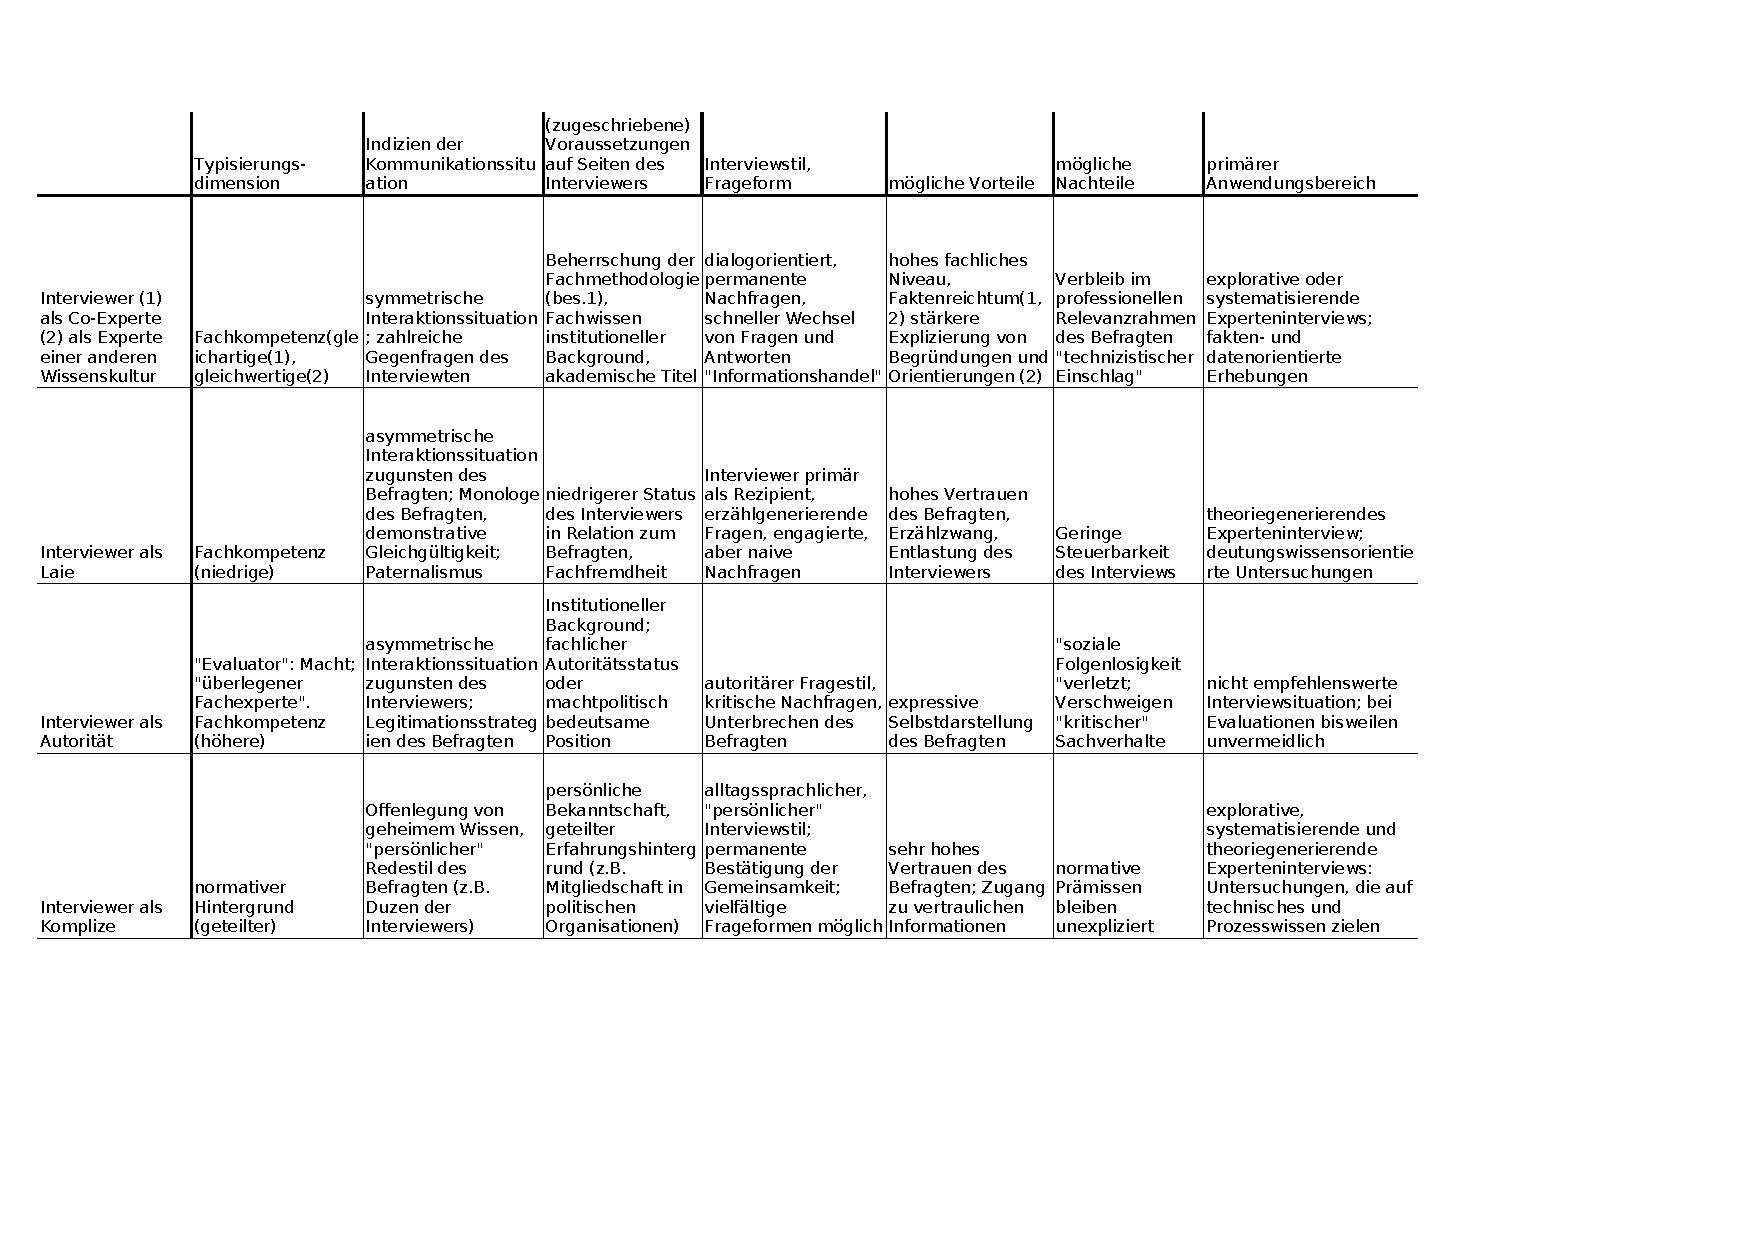
\includegraphics[width=7in,trim=0 100 0 0]{Material/Interviewsituationen.pdf}
\scriptsize{Quelle: \cite{bogmenz}: 63.}
\end{figure}
Aus dieser tabellarischen Übersicht wird deutlich, dass der Interviewer in der Interviewsituation eine oder mehrere Rollen einnimmt, bzw. vom Interviewten in unterschiedlichen Rollen wahrgenommen wird. Dies geschieht meist unbewusst und hängt von verschiedenen Faktoren ab. Da sich diese Wahrnehmung aber ggf. auf die Ergebnisse auswirkt, ist es hilfreich sich als Interviewer über die jeweils eingenommenen Rollen oder Rollenzuschreibungen klar zu werden. \par
In der von der Verfasserin durchgeführten Befragung entstand bei der Interviewerin der Einduck, dass sie von den Experten vornehmlich in einer Position wahrgenommen wurde, die zwischen den beiden Polen Co-Experte und Laie der obigen Einteilung oszillierte. Um Beeinträchtigungen des Ergebnisses der Expertenbefragung durch unterschiedliche Interviewer und deren unterschiedliches Verhalten zu vermeiden, hat die Verfasserin alle Interviews anhand eines strukturierten Gesprächsleitfadens selbst durchgeführt und selbst transkribiert.\par
Die für die vorliegende Arbeit verwendeten Interviews wurden in einem Fremdsprachenkontext durchgeführt. Die Interviewerin und der Interviewte hatten in 10 der 12 Fälle nicht die gleiche Muttersprache und auch hinsichtlich des unterschiedlichen kulturellen Kontextes ergibt sich eine besondere Situation. Die besondere Problematik hinsichtlich des kommunikationstheoretischen und analytischen Umgangs in der Durchführung und Auswertung von Interviews im fremdsprachlichen Kontext wurde in der Literatur methodisch noch kaum bearbeitet (vgl. \cite{kruse}: 121). Um eine gemeinsame Kommunikationsbasis herzustellen, wurden die Interviews auf Englisch durchgeführt, anhand eines ebenfalls auf Englisch ausgearbeiteten Leitfadens\footnote{Das Interview mit dem Official in Montenegro wurde mit einem Übersetzer für Englisch durchgeführt, da die Interviewerin kein Serbo-Kroatisch und der Interviewte kein Englisch sprach. Die Durchführung des Interviews unterschied sich von den anderen durchgeführten Interviews nur durch die Anwesenheit eines Übersetzers, der die Fragen und Antworten konsekutiv übersetzte.}. Während dieses Zurückgreifen auf eine gemeinsame Drittsprache einerseits problematisch ist, sieht Kruse auch einen möglichen Vorteil in dieser Sprachwahl-Konstellation. Während der Befragte auf der einen Seite eine Einschränkung seines gewohnten Sprachausdrucks erlebt, eröffnet sich ihm auf der anderen Seite gleichzeitig auch die Freiheit, sich außerhalb der gewohnten idiomatischen Systeme der Muttersprache auszudrücken (vgl. \cite{kruse}: 123). \par
Als Zeitschätzung, die auch in einem Probeinterview getestet wurde, war eine Stunde zur Durchführung eines Interviews vorgesehen. Während diese Zielvorgabe für die Mehrzahl der Interviews eingehalten wurde, dauerte ein Interview nur knapp 30 Minuten, zwei Interviews dauerten dagegen länger als eineinhalb Stunden. Die Fragen wurden den Interviewten nicht vor dem Interview zur Verfügung gestellt und auch nicht schriftlich vorgelegt. Alle Interviewten beantworteten die Fragen am Tag des Interviews, ohne diese vorher zu kennen. Die Interviews wurden mit einem digitalen Aufnahmegerät aufgezeichnet. Ein Interview wurde nicht aufgenommen, weil der Interviewte Vorbehalte gegen die Aufzeichnung hatte. In diesem Fall wurde eine handschriftliche Mitschrift durch die Interviewerin angefertigt. Alle transkribierten Interviews in ganzer Länge sowie die von der Autorin vorgeschlagene Auswahl an Textstellen zur Weiterverarbeitung im Forschungszusammenhang wurden der/dem jeweils Interviewten zugesandt und von ihm/ihr autorisiert. Jedem Interviewten wurde nur ihr/sein eigenes Interview vorgelegt.\par
Die durchgeführten Interviews wurden von der Autorin, unter Beibehaltung der englischen Sprache transkribiert. Dieses Vorgehen wurde gewählt, um Interpretations- und Deutungsverluste durch eine Übersetzung zu vermeiden. Aus dem gleichen Grund wurden die Interviews nicht in die deutsche Sprache übersetzt. Eine Zusammenstellung der für die Auswertung ausgewählten Interviewabschnitte ist als Kompilation pro Frage in Anhang xx TODO:ref beigefügt.

\subsection{Auswertung der Interviews}
Für die Auswertung des gewonnenen Materials hat sich in der qualitativen Sozialforschung eine Reihe von Methoden und Verfahren herausgebildet, die meist ohne Systematisierung nebeneinander gestellt und unabhängig voneinander beschrieben werden. Von Gläser / Laudel werden unterschieden:
\begin{itemize}
\item Freie Interpretation
\item Sequenzanalytische Verfahrensweise
\item Grounded theory (Kodieren)
\item Qualitative Inhaltsanalyse
\end{itemize}

\begin{figure}
\caption{Überblick zu Verfahren der Interviewauswertung in den Sozialwissenschaften}
\includegraphics[width=5in]{Material/KlassifizierungAuswertungsmethoden}\\
\scriptsize{Quelle: \cite{glalau10}: 44}
\end{figure}
Die Abbildung veranschaulicht die vier Wesentlichen in den Sozialwissenschaften angewandten Methoden der Auswertung von Interviews.\par
Die freien Interpretationen sind in der Forschungspraxis weit verbreitet, es besteht dabei allerdings die Gefahr, dass die Ergebnisse nicht nachvollzogen werden können. Auch gibt es kaum Verfahrensregeln für diese Herangehensweise. Kritisch wird von „stillschweigender Verkodung“ (vgl. \cite{hopf}: 316) gesprochen.\par
Bei der sequenzanalytischen Verfahrensweise werden die thematischen und zeitlichen Verknüpfungen der in den Texten enthaltenen Aussagen analysiert. Als wichtigste Methoden gelten die Narrationsanalyse und die objektive Hermeneutik. Die Narrationsanalyse nach Schütze betrachtet die Anordnung und Verknüpfung von Textabschnitten und Textsorten und kommt auf dieser Grundlage zu analytischen Aussagen. In der objektiven Hermeneutik nach Oevermann werden zunächst alle denkbaren Interpretationen entwickelt, die daraufhin auf ihre Übereinstimmung mit dem Text überprüft werden (vgl. \cite{glalau10}: 45).\par
Auf der Basis einer anderen komplexen Herangehensweise, der grounded theory\footnote{In der vor allem in der anglo-amerikanischen Forschung entwickelten ‚grounded theory’ werden Fallauswahl, Erhebungs- und Auswertungsmethoden in einem zyklischen Prozess miteinander verkoppelt. Empirische Ergebnisse und Erfahrungen führen zu neuen Überlegungen und zur Fallauswahl sowie der Beobachtungsstrategie, was wiederum zu neuen empirischen Daten führt, usw. (vgl. \cite{glalau10}: 47).}, hat sich das ‚Kodieren’ zu einer eigenständigen Auswertungsmethode entwickelt. Dabei werden Textstellen mit für das Thema relevanten Informationen mit einem Kode markiert. Diese Kodes werden für den gesamten Text gesetzt und im Ergebnis entsteht eine Art Struktur des Textes. Aufgrund dieses Rasters sind Bedeutungen zu erkennen und darauf aufbauend wird die Analyse und Beantwortung der Forschungsfrage vorgenommen (vgl. \cite{kruse}: 163ff.).\par
Für Experteninterviews wird vorwiegend mit einem anderen Verfahren, dem der qualitativen Inhaltsanalyse gearbeitet. Dabei werden in einem systematischen Verfahren Informationen aus dem Text entnommen. Die Texte werden mit einem Analyseraster auf relevante Informationen hin durchsucht und die entsprechenden Textstellen in die Analysekategorien eingestellt. Diese werden daraufhin relativ unabhängig vom Interviewtext weiterverarbeitet und mit anderen Informationen synthetisiert. Bei diesem Verfahren bleibt der Bezug zum Text zwar über eine Quellenangabe erhalten, die weitere Analyse wird aber mit den aus dem Text extrahierten Informationen durchgeführt (vgl. \cite{glalau10}: 46). In der vorliegenden Arbeit wird mit diesem Verfahren der qualitativen Inhaltsanalyse gearbeitet. \par
Das Verfahren wird in vier Schritte untergliedert, die nacheinander durchgeführt werden:
\begin{itemize}
\item das Aufbauen eines geschlossenen Kategoriensystems vor der Analyse,
\item das Zerlegen des Textes in Analyseeinheiten,
\item das Durchsuchen des Textes auf relevante Informationen und
\item die Zuordnung dieser Informationen zu den Kategorien (vgl. \cite{glalau10}: 198).
\end{itemize}
Das Ziel dieser Verfahrensweise ist die Extraktion der wesentlichen Informationen aus dem Text der Experteninterviews. Die Gesamtgestalt der Erzählung und die Struktur des Textes werden, anders als bei der Biografieforschung, nicht für die Analyse herangezogen (vgl. \cite{glalau10}: 204).\par
In der Vorgehensweise der qualitativen Inhaltsanalyse werden die einzelnen Interviews zunächst auf die dargestellten Zusammenhänge hin untersucht. In einem nächsten Schritt wird dann untersucht, ob es Gemeinsamkeiten und Unterschiede zwischen den dargestellten Fällen gibt. Entsprechende Fragen dazu sind:
\begin{itemize}
\item Welche Faktoren treten in allen Fällen auf, welche nur in einigen?
\item Welche Faktoren treten überraschend auf (wurden nicht erwartet), welche Faktoren fehlen? (vgl. \cite{glalau10}: 249).
\end{itemize}
In der folgenden Auswertung wird nach diesem Muster der qualitativen Inhaltsanalyse vorgegangen.

\section{Wesentliche Ergebnisse der Expertenbefragung }
Die Ergebnisse der Befragung von EU-Offiziellen in Brüssel und eines OECD/SIGMA-Vertreters in Paris auf der einen sowie die Ergebnisse der Interviews mit je einem Vertreter der Regierung und einem Vertreter einer NGO in den Untersuchungsländern auf der anderen Seite werden im Folgenden in prägnanten Themenblöcken dargestellt, die inhaltlich den Themenbereichen aus dem Interviewleitfaden entsprechen.\par

Unterschieden werden:
\begin{itemize}
\item Themen und Stellenwert der Verwaltungsentwicklung
\item Bedingungen für die Verwaltungsentwicklung
\item EU-Programme zur Förderung der Verwaltungsentwicklung
\item Projektmanagement der EU zur Verwaltungsentwicklung
\item Perspektiven für die Verwaltungsentwicklung und den EU-Beitritt
\end{itemize}
\section{Stellenwert der Verwaltungsentwicklung }
Die befragten Experten sind sich einig, dass Verwaltungsmodernisierung ein wichtiges Thema im Rahmen des Erweiterungsdialoges mit den einzelnen Ländern sein muss. Sie beantworteten folgende Frage zum Zusammenhang Verwaltungsmodernisierung und Acquis communautaire:
\begin{itemize}[label={}]
\item \ul{Public Administration Reform is not a separate chapter in the Acquis. Should it be a separate chapter? }
\end{itemize}

Die Meinungen zu dieser Frage, ob angesichts der Wichtigkeit des Themas ein eigenes Kapitel im Acquis eingerichtet sollte, gehen allerdings auseinander. Eine Sichtweise ist die, dass es unlogisch und gewissermaßen unfair wäre für zukünftige Erweiterungen Verwaltungsmodernisierung als eigenes Kapitel in den Acquis aufzunehmen, weil dadurch eine Ungleichbehandlung gegenüber früheren Beitritten hervorgerufen würde. Stellvertretend für diese Sichtweise:
\begin{itemize}[label={}]
\item \textit{“It is part of the political criteria and that suffices. It has been the case for all countries joining the EU, why should it be different for Macedonia” (NGO representative Macedonia, Frage 4).
}
\end{itemize}
Als Begründung gegen ein eigenes Kapitel im Acquis wird häufig die Sichtweise von Verwaltungsmodernisierung als nationaler Angelegenheit angeführt. Diese sei eher eine horizontale Aufgabe, im Gegensatz zu den vertikalen Themen des Acquis communautaire. Die EU könne und solle daher keinen direkten Einfluss nehmen.

\begin{itemize}[label={}]
\item \textit{“Of course it should not be a separate chapter. If there should be a chapter, it should be with the word horizontal in brackets. I think it always comes out again that horizontal PAR is a domestic issue and not something the EC should get too involved in”(EU official, DG ELARG Evaluation Unit team, Frage 6). }
\end{itemize}

Neben der Einordnung der Verwaltungsmodernisierung als horizontaler Aufgabe im Erweiterungsprozess wird in diesem Zusammenhang auch oft von „weichem“ Acquis gesprochen, denn bei der Verwaltungsmodernisierung handelt es sich nicht um Forderungen, die sich direkt aus der EU-Gesetzgebung und -Richtlinien ableiten. 
Ein weiteres Argument gegen ein eigenes Acquis-Kapitel ist der unterschiedliche Aufbau von nationalen öffentlichen Verwaltungen. Ein Kriterienkatalog bezüglich Verwaltungsmodernisierung würde die Mitgliedstaaten auf den Plan rufen, so eine Meinung, da die Verwaltungsausgestaltung als ausschließlich nationale Angelegenheit wahrgenommen wird:
\begin{itemize}[label={}]
\item \textit{„Some of these chapters or even the majority are not necessarily based on hard Acquis, EU legislation, EU directives and so on. Some of the chapters appear to be soft in character, meaning that they sometimes refer to international agreements, standards, conventions or treaties issued by other bodies, such as the CoE. The issue of creating a new chapter on PAR is currently not realistic because there are complex legal and procedural matters and there was also a feeling that it would not be right to add a new chapter as if we would make it more difficult for the new candidate countries compared to the previous ones. Also, there was the argument that perhaps the member states, who would decide on the change in the Acquis might object, because it has at least indirect implications for them. How does it look like if we in a chapter request certain PA reforms, which perhaps are not in place in the MS themselves?”(EC official, DG ELARG PAR Coordination team, Frage 6).}
\end{itemize}

Anhand des Beispiels des Konzeptes von Public Internal Financial Control (PIFC), das Eingang fand in eines der Acquis-Kapitel, wird von einem Gesprächspartner auf die Probleme mit ambitionierten Reformansätzen der öffentlichen Verwaltung hingewiesen. Diese führen teilweise zu Lösungen, die nicht an die nationalen Gegebenheiten angepasst sind und Ressourcen binden:
\begin{itemize}[label={}]
\item \textit{„So one part of the answer is that I do not think you could make it a chapter and my position is to some extent re-enforced by the leading example of what we have been talking about, which is PIFC, which is absolutely not Acquis. It was negotiated into a chapter, now chapter 32. The result in my view was that many of the countries were forced to create systems they could not find models of elsewhere; which were not appropriate or sustainable and which diverted scarce resources into low priority tasks and away from consolidating basic systems. I think it would be far more powerful for the Commission, if it simply relied on the political chapter and ensured that the political chapter was not forgotten about, as soon as negotiations started”(OECD/SIGMA team, Frage 6).}
\end{itemize}

Die Problematik von propagierten Lösungen, die nicht den nationalen Gegebenheiten gerecht werden, erwähnt einer der nationalen Experten aus Montenegro ebenfalls. Die EU fordere oder empfehle mitunter Maßnahmen im Bereich öffentliche Verwaltung, die der Größe des Landes nicht angemessen sind:
\begin{itemize}[label={}]
\item \textit{„The issue of the organization of the public administration and its reform is specific and it seems that there are no principles or guidelines that can be universally applied. The issue of forming independent regulatory bodies, independent from the state administration, that is the main pre-condition of the EU. Montenegro is requested to form these independent regulatory bodies and over the past 7 or 8 years the number of such bodies doubled. We had 40 or so, but now we have 100. And there is the issue of functionality. And then SIGMA comes asks why have you done this? Montenegro has a population of 650,000. It is not possible for Montenegro to copy anybody else’s experience, because we are such a small country” (Official, Montenegro, Frage 4).}
\end{itemize}

Neben diesen Beispielen, die gegen eine Aufnahme der Verwaltungsreform in den Acquis sprechen, sind andere Meinungen vertreten, die eine stärkere Konzentration auf Verwaltungsmodernisierung für wünschenswert halten und Verwaltungsreform als eigenes Kapitel in den Acquis aufgenommen sehen wollen oder das Thema zumindest in den Verhandlungen stärken wollen, wie in den folgenden Auszügen deutlich wird:
\begin{itemize}[label={}]
\item \textit{„So maybe it is a good idea to have a separate chapter, in order to have even more pressure” (Official Albania, Frage 4).}

\item \textit{ „I think it should be a chapter in negotiations (as there is no acquis in this area) and dealt with separately, not only as part of each chapter” (NGO representative Albania, Frage 4).}

\item \textit{„But even in the absence of a formal chapter, we can increase the profile of PAR. That means to really discuss it, to conduct a political dialogue with the candidate countries as we do with the chapters” (EC official, DG ELARG PAR Coordination team, Frage 6).}
\end{itemize}

Die Entwicklung einer PAR checklist5 durch die EU im Jahr 2010 und die Einrichtung einer speziellen Arbeitsgruppe zur öffentlichen Verwaltung in Mazedonien, ebenfalls im Jahr 2010, werden als Beispiele genannt, um zu belegen, dass der Verwaltungsmodernisierung im Rahmen der Erweiterungsdiskussion ein zunehmend hoher Stellenwert zukommt:

\begin{itemize}[label={}]
\item \textit{„The EC has drafted a checklist recently on PAR. This very fact is driven by the dilemma on whether there should be a chapter or not…Thus in the progress reports, as Brussels is always evaluating the administration, there should be a chapter. The first step in that direction is already done. I do not know if you are aware that Macedonia is the first candidate country with a special working group on PA. The special working group is at the level of a sub-committee” (Official Macedonia, Frage 4).}
\end{itemize}

Die Meinungen zur Frage, ob Verwaltungsmodernisierung Eingang in den Acquis finden sollte, gehen stark auseinander. Allerdings sind sich alle Befragten einig über die große Bedeutung dieses Themas für die Zusammenarbeit Brüssels mit den (potenziellen) Kandidatenländern im Erweiterungsprozess. Von mehreren Gesprächspartnern wurde auch betont, dass ein „Dranbleiben“ der EU am Thema Verwaltungsmodernisierung notwendig sei, insbesondere nach der Eröffnung der Beitrittsverhandlungen, wie z.B. folgende Aussage verdeutlicht:

\begin{itemize}[label={}]
\item \textit{„Should it be a separate chapter, I don’t know. If it would be a separate chapter, it would take out from other chapters and that would not be possible, thus I would say no, but should it be strengthened also in the chapter parts? There, I would say yes. We also have to find guidance and incentives after the opening of negotiations and not stop after we evaluated it. PAR is an overall process and does not stop there” (EC official, DG ELARG Albania team, Frage 6).}
\end{itemize}

Für eine Perspektivenverschiebung weg von Input-Indikatoren hin zu einer Outcome-Orientierung bei der Betrachtung von Verwaltungsmodernisierung im Erweiterungsprozess plädiert der Interviewpartner der OECD/SIGMA:

\begin{itemize}[label={}]
\item \textit{„Also, I would like to start thinking about outcome measures, for example on administrative reliability. What sort of indicators should we have to measure if administration is acting in a reliable and impartial way? You have for example the analysis of judgements of administrative courts, you have the ombudsman. You could imagine a number of different methods, case based sampling, customer surveys etc. I would like to see a move towards an approach, where we do not say what the inputs are, but what we would like to be the outputs” (OECD/SIGMA team, Frage 6).}
\end{itemize}


In den Antworten der Experten wird PAR im Rahmen der politischen Kriterien im Erweiterungsprozess verortet. Deutlich wird dabei, wie in früheren Kapiteln dieser Arbeit dargestellt, dass PAR kein direkter Bestandteil des Acquis ist mit ableitbarem Kriterienkatalog. Dennoch wird PAR von den Experten als sehr wichtig eingeschätzt im Sinne eines Leitbildes, als horizontale Aufgabe und Voraussetzung einer erfolgreichen Umsetzung des Acquis. Auch die Einordnung als Governance-Thema (siehe Einleitung) wird deutlich, wie die beiden folgenden Zitate exemplarisch belegen: 

\begin{itemize}[label={}]
\item \textit{„PAR or governance is a key priority of the enlargement process…Mostly priorities related to PAR are found under political criteria and there we have them under Parliament, Government and PA, but also under headings such as political rights, anti-corruption and possibly under Chapter 23 (Judiciary and Fundamental Rights) or Chapter 32 (Financial Control)” (EC official, PAR Coordination team, Frage 1).}
\item \textit{„PAR is an overarching horizontal aspect that goes beyond the political criteria, but that is reflected specifically in the political criteria and PAR is an issue for Albania” (EC official, DG ELARG Albania team, Frage1).}
\end{itemize}

Ebenfalls wird die noch allgemeinere Einbindung in das Konzept der Demokratisierung vorgenommen:
\begin{itemize}[label={}]
\item \textit{„One of the goals is to install democratic stability in these countries with functioning institutions. The institutions we focus on are very much in the sector of Justice and Home Affairs and institutions linked to democratic stability“ (EC official, DG ELARG, Evaluation Unit team, Frage 1).}
\end{itemize}

Zusammenfassend ist festzustellen, dass alle Interviewpartner auf die große Bedeutung von Verwaltungsentwicklung/Verwaltungsreform im Erweiterungsprozess verweisen. Es wird deutlich, dass die fehlende Verankerung im Sinne eines Acquis-Kapitels ein Dilemma darstellt, das sich in den kontroversen Antworten zur Frage der Einführung eines entsprechenden Acquis-Kapitels widerspiegelt. Einerseits wird argumentiert, man solle für die jetzigen Aufnahmekandikaten nicht andere Bedingungen schaffen als für die früheren Kandidaten, andererseits wird die Meinung vertreten, Verwaltungsmodernisierung sei ein so zentrales Thema, dass ein separates Acquis-Kapitel nötig sei und zusätzlich ein Monitoring noch nach der Aufnahme in die EU.

\subsection{Verwaltungsmodernisierung = Civil Service Reform }
In der Auswertung der Interviews wird die Wahrnehmung der befragten Experten zum Stand der Verwaltungsentwicklung in den Untersuchungsländern betrachtet. Dabei interessiert zum einen die Darstellung des Status quo durch die Experten. Dies ist die Einstiegsfrage im Interviewleitfaden für alle Interviewten. Zum anderen interessieren für die weitere Untersuchung auch Unterschiede zwischen den EU officials und den nationalen Experten vor Ort in der Prioritätensetzung und in der Einschätzung zum Status quo der Verwaltungsentwicklung im Westlichen Balkan. 

Die Experten der EU und der OECD beantworteten im genannten Zusammenhang folgende Frage\footnote{Die komplette Liste aller Fragen, die den Experten der EU und OECD in Brüssel und Paris gestellt wurden, ist in Anhang x TODO:ref aufgeführt.}:
\begin{itemize}[label={}]
\item \ul{Which topics/areas are presently dealt with as a priority by the EU regarding Public Administration Reform in Albania, Macedonia, Montenegro? What are the developments you see there?}
\end{itemize}

Die Experten in den drei Untersuchungsländern wurden gebeten, diese Frage jeweils bezogen auf ihr Land zu beantworten\footnote{Die komplette Liste aller Fragen, die den Experten in den Untersuchungsländern gestellt wurden, ist in Anhang x TODO:ref aufgeführt.}:
\begin{itemize}[label={}]
\item \ul{Which main topics/areas in the context of Public Administration Reform are presently dealt with as a priority by Albania, Macedonia, Montenegro?}
\end{itemize}

In der Auswertung fällt auf, dass in den Antworten auf die Frage nach den aktuellen Prioritäten der Verwaltungsentwicklung im Westlichen Balkan fast ausschließlich der civil service als Bereich benannt wird, auf den sich das Augenmerk richtet. Andere Themen der Verwaltungsmodernisierung, wie z. B. die Einführung von Controlling, Kundenorientierung oder Evaluierung wurden, insbesondere von den interviewten EU officials, generell nicht benannt. \par
Als wesentliches Thema der Reform der öffentlichen Verwaltung in den Untersuchungsländern sehen die Interviewpartner vor allem den Öffentlichen Dienst (civil service), der als unabhängig von politischen Interessen zu organisieren ist, was bisher nur in Ansätzen gelungen sei:
\begin{itemize}[label={}]
\item \textit{„The main priority in all the countries is to establish a civil service and a PA that is professional and not influenced by political constellations. There is a tendency, especially after elections to replace many people in the PA” (EC official, DG ELARG PAR Coordination team, Frage 1). }
\item \textit{„The main topic now is related to civil service law and that is the topic of recruitment, the principle of recruitment based on merit and on a transparent process. We also saw overuse of so called temporary employments, which might be a specific case for Macedonia. The state administration for whatever capacity they needed would get staff through private employment agencies for one year on a short term contract to do the job of a civil servant. In summer 2010, the authorities of Macedonia started the process of recruitment and there are indications that not everything was as transparent as it should be. And there are signals that those who were temporarily employed were given an advantage, if they were not directly transferred, which is of course against the principles” (EC official, DG ELARG Macedonia team, Frage 1).}
\item \textit{„In our view PAR in Albania is incomplete; there are certain issues we are following up very closely and in detailed discussions and exchanges with SIGMA. We are fully in line with the analysis SIGMA is providing in this regard on the ongoing process of civil service law reform in Albania and strengthening the department that deals with that reform. These are priorities for us in terms of financing” (EC official, DG ELARG Albania team, Frage 1). }
\item \textit{„Priorities are mainly in the filed of civil service, training issues and the non-political recruitment of civil servants in every ministry. Non political civil servants still needs to improve in Montenegro” (EC official, DG ELARG Montenegro team, Frage 1).}
\end{itemize}
Neben dieser auffälligen Betonung des Themas civil service wird von den EU officials die fehlende Implementierung von Gesetzen genannt. Weitere Nebenthemen sind die notwendige institutionelle Einbindung und die Koordinierung der Verwaltungsmodernisierung bei einer verantwortlichen Institution in den Untersuchungsländern.\par
Auch für die Interviewpartner aus den Untersuchungsländern steht die Reform des civil service im Vordergrund bei der Frage nach den aktuellen Themen der Verwaltungsreform in ihren Ländern. Und auch dort sehen die Interviewpartner es als wichtiges Ziel an, die politische Einflussnahme bei der Rekrutierung von Personal zu beschränken:
\begin{itemize}[label={}]
\item \textit{„We are working on two laws at the moment. One is on civil service. The one in place is from 1999 and a 3/5th majority in parliament is needed to change it. There are pitfalls within the existing law and now after 11 years we see that there are a lot of problems with implementation. The other law is the law on organization and functioning of public administration” (Official, Albania, Frage1)}
\item \textit{„Reforming the public administration has always been a pre condition for other reforms to be implemented and to be pushed forward in the European Integration Process, which is the driving force or at least should be the driving force of reform in Albania… The law on civil servants is in many parts not properly implemented, e.g., the removal of persons from office is not based on proper argumentation and reasons. Most of the time, replacements were done for political reasons, in particular when a new political force comes into place, but we have seen that it also takes place when there is a change of the head of a Ministry or independent institution. The problem is not the law, but the mentality of dealing with this issue and that is the biggest concern. Also, a lot of judicial decisions withholding the requests of former employees are not implemented by state institutions” (NGO representative, Albania, Frage 1).}
\item \textit{„We have 10.000 civil servants at central level and 3.000 at local level. This is one tenth of the whole number of approx 100,000 public employees. The government just adopted a new PAR strategy at the end of 2010. The main focus will be on the further professionalization and depolitization of the PA“ (Official, Macedonia, Frage 1).}
\item \textit{„For 2011 it is the new PAR strategy, which was developed in the context of an EU project. It will be the main co-ordinator of the Public Administration Reform process in the country. All the duties that used to belong to the Civil Servants Agency are envisaged to be transferred to a new ministry, the ministry of Administration and Information Technology” (NGO representative, Macedonia, Frage 1).}
\item \textit{„In the area of Public Administration with the new AURUM strategy adopted by Parliament, rationalization of the PA structure, stabilization of public finance including external and internal financial control, the area concerning the personnel system with implementation of a merit system and a completely new law on public officials” (Official, Montenegro, Frage 1). }
\item \textit{„From 2003 to 2009 we had a PAR strategy. The drafting and implementation of the strategy was financed by the EU through PARIM I and II projects. Most of that was completed in 2007/8, drafting of new legislation on state administration, state employees, the organization etc. Between 2008 and today, 2011 little was done. The work on the new strategy started at the end of 2009 officially. While we do not have the document yet, a first version was consulted with civil society, SIGMA, CoE and UNDP. In the last quarter of the last year we had preparations for government changes. Preparations for the new president of this gov’t, new structures, new ministers, and the new PAR strategy was waiting for the new structure to adopt it” (NGO Representative, Montenegro, Frage 1) . }
\end{itemize}


In der folgenden Antwort schwingt eine gewisse Enttäuschung angesichts der wiederkehrenden Kritik aus Brüssel am politisierten civil service mit, ebenso eine gewisse Resignation angesichts der Tatsache, dass sogar eine eigens eingerichtete Institution zur (unpolitischen) Rekrutierung von Personal, der Politisierung nicht Einhalt gebieten konnte\footnote{Zu Ende 2010 wurden wesentliche Kompetenzen der Civil Servants Agency (CSA), dem nun neu mit der Aufgabe der PAR-Koordination beauftragten Ministerium für Verwaltung und Informationstechnologien übertragen.}. 
\begin{itemize}[label={}]
\item \textit{„Every year we receive from Brussels the criticism about the politisation of the administration, which exists in reality; we can not deny it especially outside of the civil service, where the rules for employment are basically non-existent. We are using the general labour code, which does not give anything in terms of criteria for selection. The head of a hospital can hire and dismiss at any time. This is not the case in the civil service, where we have since 2000 very precise and detailed regulations. Unfortunately, even there, the Civil Servants Agency (CSA) was not able to defend the system from political influence. In particular during the past years, this political influence has become enormous and the CSA has failed to defend the system from this type of interference“(Official, Macedonia, Frage 1).}
\end{itemize}
Auch die Interviewpartner aus den Untersuchungsländern sehen die Weiterentwicklung des civil service als Hauptthema der Verwaltungsmodernisierung. Weiterhin beziehen sich in den Untersuchungsländern fast alle Interview-Antworten auf die Notwendigkeit einer PAR-Strategie bzw. Einbindung in eine größere Reformdebatte, die als wünschenswert erachtet wird. Eine solche Rückbindung der aktuellen Themen von PAR an strategische Papiere oder Debatten sprechen die EU officials mit einer Ausnahme nicht an\footnote{Eine PAR-Strategie wird lediglich von einem Interviewpartner erwähnt: (Frage 1: EC official DG ELARG Montenegro).}. Alle in den Untersuchungsländern befragten Interviewpartner hingegen erwähnen die bestehende oder erwünschte Einbindung in eine PAR-Strategie. Dies ist insofern überraschend, als man die Forderung einer Anbindung der Verwaltungsmodernisierung an eine Strategie eher von der EU-Seite erwartet hätte.\par
Möglicherweise ist der Rekurs auf eine in einer Strategie definierten Zielvorgabe angesichts der wenig greifbaren Ergebnisse der Verwaltungsmodernisierung oder eines nicht vorhandenen EU-Modells wünschenswert für die Gesprächspartner in den Untersuchungsländern. Eine andere Erklärung wäre, dass die Interviewpartner in den Untersuchungsländern häufig für Fortschrittsberichte oder andere Dokumentationen der EU oder SIGMA den Reformstand beschreiben müssen und gewohnt sind, innerhalb dieses Berichtswesens strategische Papiere zu erwähnen.\par
Andere Themen, die neben dem überwiegend genannten civil service erwähnt werden, sind die Etablierung einer Verwaltungsgerichtsbarkeit und die Weiterentwicklung des Verwaltungsprozessrechtes für Albanien. Der Regierungsvertreter Montenegros benennt externe und interne Finanzkontrolle, Verwaltungsprozessrecht, One-Stop Shops, Koordinierung nationaler policies sowie die Qualität von Gesetzgebung mit Gesetzesfolgenabschätzung, zeitliche Befristung von Gesetzen und Beteiligung der Zivilgesellschaft (NGOs) im Gesetzgebungsprozess:
\begin{itemize}[label={}]
\item \textit{„In the area of Public Administration with the new AURUM strategy adopted by Parliament, rationalization of the PA structure, stabilization of public finance including external and internal financial control, the area concerning the personnel system with implementation of a merit system and a completely new law on public officials. Other developments are one stop shop reform and a new law on Admin Procedure, the issue of the quality of laws, and strategic documents. In this area, especially the coordination of national policies was emphasised, introducing regulatory impact assessments, and regulation guillotine, and the issue of NGO participation in drafting the documents. We are often copying the solutions from the EU, but we do not have a systemic approach to deal with these issues” (Official, Montenegro, Frage 1).}
\end{itemize}
Die hier erwähnten Elemente stellen konkrete Ziele aus der Debatte um Verwaltungsmodernisierung in Zusammenhang mit dem Konzept des New Public Management (NPM) dar. Interessanterweise kommen diese Überlegungen aus dem kleinsten der Untersuchungsländer, das aufgrund seiner Größe besonders mit den strukturellen Anforderungen an eine moderne öffentliche Verwaltung zu kämpfen hat. Gleichzeitig gibt der Interviewpartner zu bedenken, dass oft Lösungen der EU kopiert werden, ohne sie systemisch umsetzen zu können. Dies weist auf mögliche Probleme bei der Übernahme von NPM-Themen für kleine und oder nicht weit genug entwickelte Länder hin.\par
Die fast ausschließliche Fokussierung auf den civil service bei den Antworten zu den Themen der Verwaltungsmodernisierung sowohl bei den EU officials als auch bei den Interviewpartnern in den Untersuchungsländern ist auffallend. Der OECD/SIGMA-Interviewpartner konstatiert, dass aus Sicht von SIGMA in der Debatte zur Verwaltungsmodernisierung im Erweiterungskontext oft eine Engführung auf den civil service stattfindet. Aus SIGMAs Sicht sollten darüber hinausgehend Themen wie Verwaltungsrecht und policy making eine größere Rolle spielen und es wird ein Konzept von Public Governance vorgeschlagen.
\begin{itemize}[label={}]
\item \textit{„There is a tendency to understand PA in terms of civil service and administrative law and to some extent policy making, lately. For PA, we think, this is too narrow. It should be Public Governance. If you are dealing with PA, it should be wider than 3 or 4 main topics. Within the EU’s definition of PA in the three countries, there is a strong interest in PAR-Strategies, in Montenegro and Macedonia and perhaps a bit less so in Albania, and in that the main focus tends to be on civil service law and anti-corruption. Lately, there is increasing interest in Admin Procedures and Admin Justice” (OECD/SIGMA team, Frage 1). }
\end{itemize}
Zusammenfassend ist auffallend, dass die Qualität der Erbringung von Aufgaben, ein wichtiges Element in der Debatte um Verwaltungsmodernisierung, wie z.B. verbesserte Kundenorientierung, Evaluierungen, dezentrale Erbringung von Aufgaben, Korruptionsvermeidung oder Transparenz, von den Interviewpartnern als aktuelle Themen der Verwaltungsmodernisierung so gut wie nicht erwähnt wurden. Bei der Suche nach Erklärungen für dieses Phänomen könnte man vermuten, dass das Konzept des New Public Management, das seit den 1990er Jahren die internationale Debatte zur Verwaltungsmodernisierung bestimmt hat, noch nicht in den Ländern des Westbalkans angekommen ist. Dieser Vermutung steht aber die Eingebundenheit der Interviewpartner in internationale Zusammenhänge und ihre Funktion an zentraler Stelle der Regierung oder NGOs entgegen. Es ist davon auszugehen, dass in diesen Funktionen die aktuellen internationalen Debatten um Verwaltungsmodernisierung bekannt sind. Im Vergleich der Antworten der EU officials, die auf jeden Fall mit dem Konzept des NPM vertraut sind, und der Experten in den Untersuchungsländern fällt auf, dass die EU officials noch ausschließlicher auf den civil service fokussieren.
\subsection{Was behindert Verwaltungsmodernisierung im Balkan? }
Mit einer weiteren Frage sollen die Einschätzungen der Interviewpartner zu den wahrgenommenen Hindernissen und zu den notwendigen Bedingungen für eine erfolgreiche Verwaltungsentwicklung erhoben werden.
\begin{itemize}[label={}]
\item \ul{In your opinion, are there obstacles to PAR in Albania, Macedonia and Montenegro? And what would be necessary for successful PAR in Albania, Macedonia and Montenegro?}
\end{itemize}
Die Fokussierung auf den civil service in den Antworten der Experten zum Gegenstand der Verwaltungsentwicklung setzt sich auch in der Einschätzung der Hinderungsgründe für eine erfolgreiche Verwaltungsmodernisierung fort\footnote{Siehe Frage 3: nationale Experten und Frage 10: EU officials.}. Einer erfolgreichen Verwaltungsmodernisierung stehen nach Einschätzung der Experten vor allem entgegen:
\begin{itemize}
\item politische Einflussnahme auf Einstellungsentscheidungen der öffentlichen Verwaltung und Klientelismus,
\item Politisierung der öffentlichen Verwaltung. Wahrnehmung der öffentlichen Verwaltung als Exekutivorgan für die Regierungspartei, 
\item fehlende Implementierung bestehender gesetzlicher Vorschriften oder gerichtlicher Entscheidungen, z.B. zum öffentlichen Dienst, 
\item eine (zu) hohe Anzahl von öffentlich Bediensteten, 
\item Korruption 
\item fehlender politischer Wille und nur deklaratives Bekenntnis zur Verwaltungsmodernisierung ohne konkrete Umsetzungsabsicht.
\end{itemize}

Die folgenden exemplarischen Aussagen von Interviewpartnern illustrieren diese Beobachtungen:
\begin{itemize}[label={}]
\item \textit{„The politicians would like to have their hands free as much as possible to appoint people from their staff, wherever they go. I have seen ministers working in one government, going from one ministry to the other and taking their staff with them. Not only political staff, but also technical staff. This makes it impossible for PA to be sustainable in the long term and also to have a proper career system implemented” (NGO representative, Albania, Frage 3) .}
\item \textit{„Largely politicised PAs are an obstacle. This will only change when the countries realize that they need a professional civil service, detached to some extent from what is going on politically. Positions are changed after elections, which is a huge obstacle to us and the brain drain related to that actually means, that there is no institutional memory” (EC official, DG ELARG Evaluation Unit team, Frage 10). }
\item \textit{„In Montenegro, although you have a multi-party system, the country has been governed by more or less the same party for many years. And because the country is so small there are very close links between the political and economic elites, which could give rise to what we call state capture, the most serious form of corruption” (EC official, DG ELARG PAR Coordination team, Frage 10).}
\item \textit{„The main obstacle is that there is continuous, declaratively announced political will for the de-politisation and further reform of the PA, but we have not seen any tangible results from any of the government structures today. For example for the rightsizing process, which has been declaratively initiated since 1999 or 2000, all the political parties that have ruled the country since then have declared, that they would decrease the number of people in the public sector. But there is no concrete strategy until now to solve the problem” (NGO representative, Macedonia, Frage 3). }
\item \textit{„I think the basic obstacle is that the people do not want it in the countries themselves… There may be demand from society, but whether political, administrative and business elites are interested in PAR, I am not so sure” (OECD/SIGMA team, Frage 10). }
\end{itemize}
Bei den Hinderungsgründen für Verwaltungsmodernisierung sind sich die Befragten weitgehend einig. Die Politisierung der öffentlichen Verwaltung wird als DER Hinderungsgrund benannt. In der Wahrnehmung der Interviewpartner wird die öffentliche Verwaltung als verlängertes Instrument der (Regierungs-)Elite des jeweiligen Landes gesehen. Bei Regierungswechseln wird nach Einschätzung der Experten fast die gesamte öffentliche Verwaltung ausgewechselt. So wird einerseits politischer Einfluss ausgeübt und andererseits Zugang zu ökonomischer Teilhabe für die Stelleninhaber ermöglicht. Mit dieser Praxis wird auch die Entstehung eines „institutional memory“ erschwert, was wiederum effektive Verwaltungsprozesse behindern kann.
\subsection{Hinderungsgründe für Verwaltungsmodernisierung im Westlichen Balkan}

Im Folgenden soll untersucht werden, ob sich über die Antworten der Interviewpartner zu den Hinderungsgründen für Verwaltungsmodernisierung hinaus weitere Erklärungen für die wahrgenommenen Probleme anbieten.\par
Als wichtiges Element wird von einigen Interviewpartnern die politische Kultur benannt, in der es keine Tradition des politischen Interessensausgleichs zum Wohl der Allgemeinheit gibt. Jede Seite versucht kompromisslos ihre Interessen durchzusetzen, was häufig zu Blockadesituationen führt.
\begin{itemize}[label={}]
\item \textit{„Albania, also a small country, has a strong historical legacy and everything is very much politicized, with limited stability in the public administration” (EC official, DG ELARG PAR Coordination team, Frage 10).}
\item \textit{„The opposition is not really interested to have the new legislation, even the municipalities run by the opposition, and most municipalities are run by the opposition. It is a kind of political culture that is blocking a lot of things here, not only this law. Apart from having good laws, we also do not have a strong culture of implementing the laws that are in place” (Official, Albania, Frage 3).}
\end{itemize}
Die politische Blockadekultur wird auch angewandt, um den Einfluss auf die Besetzung von Stellen in der öffentlichen Verwaltung nicht aus der (politischen) Hand geben zu müssen, wie zwei Beispiele von Experten aus den Untersuchungsländern zeigen:
\begin{itemize}[label={}]
\item \textit{„In terms of professionalizing, we were 2-3 years ago proposing to establish senior civil service, to establish also fast tracking mechanism for juniors for their advancement in their career. It was not accepted, because establishment of senior civil service would mean that the interference of politics would be dramatically decreased. And politicians still are not willing to give up on these tools” (Official, Macedonia, Frage 3).}
\item \textit{”There is a lot of invisible struggle, for example, on the solution of unifying the inspection controls of all the ministries into one. Now there is the situation where a minister has to give up his inspections, or the solution of one stop shops for issuing permits. But that for a minister means that he does not have a say in giving out permits in certain areas. That is why certain government officials do not look favourably upon these reforms and the excuse they are using is the failure of similar reforms in other countries” (Official, Montenegro, Frage 7).}
\end{itemize}
Als ebenso kulturell verortet wird die fehlende Implementierung von Gesetzen gesehen, die als einer der Hinderungsgründe für Verwaltungsmodernisierung benannt wird.
\begin{itemize}[label={}]
\item \textit{„Necessary for successful PAR would be strengthening the implementation of laws. While the laws have undergone a lot of changes, still the EU and the experts say the legal framework is good, and an EU approximated one and that it can and should ensure the proper functioning of the PA and the civil service. But as we know we always have this weakness of implementation of legislation in general in the country” (NGO representative, Macedonia, Frage 3).}
\item \textit{„An obstacle certainly is culture. The strong sense of authority of the highest person and non-transparency has to change” (EC official, DG ELARG Albania team, Frage 10).}
\end{itemize}
Die Interviewpartner sowohl aus den EU-Strukturen als auch aus den Untersuchungsländern sind sich weitgehend einig darin, dass die Gründe für die beschriebenen Probleme der Verwaltungsmodernisierung primär im kulturellen Bereich anzusiedeln sind.\par
Es wird deutlich, dass kulturelle Gründe für die Probleme im Bereich der Verwaltungsmodernisierung als wesentlich benannt werden. Kulturelle Prägungen sind langfristiger Natur und haben mit der geschichtlichen Verortung der Verwaltung zu tun. Das heißt, nicht nur die Verwaltungsentwicklung der neuesten Zeit sind zu betrachten. Vielmehr ist es notwendig, die Einflüsse aus der Zeit vor dem Einsetzen der demokratischen Entwicklung mit einzubeziehen. Nur unter Einbeziehung dieser historischen Perspektive kann eine adäquate Herangehensweise an die Verwaltungsentwicklung in den Untersuchungsländern innerhalb der weiteren EU-Annäherung entwickelt werden. Doch bevor hierzu die Rückbeziehung auf die Erkenntnisse aus den historischen Kapiteln dieser Arbeit im Abschlusskapitel erfolgt, sollen weitere Themen der Experteninterviews ausgewertet werden, die für die Gesamtbetrachtung wichtig sind: Die EU-Pro"-gramme zur Förderung der Verwaltungsmodernisierung, das Projektmanagement der EU zur Verwaltungsmodernisierung und die Perspektiven für die Verwaltungsentwicklung und den EU-Beitritt.

\subsection{Voraussetzungen für erfolgreiche Verwaltungsmodernisierung }
Mehrere Interviewpartner boten Lösungsansätze zur Förderung der Verwaltungsentwicklung an. Dabei wurden vor allem konkrete Maßnahmen genannt, wie z.B. die Einführung von Leistungsbeurteilungen und eine generelle Outcome-Orientierung:
\begin{itemize}[label={}]
\item \textit{„Heads of local institutions should feel that they would be judged for what they produce and the outcome of their work. Then they would feel the need to have proper administration in the institutions established and working professionally” (NGO representative, Albania, Frage 3).}
\end{itemize}
Auch Weiterbildungsmaßnahmen für die Beschäftigten der öffentlichen Verwaltung und einer stärkeren Beteiligung gesellschaftlicher Gruppen an der Entwicklung von Strategien zur Verwaltungsmodernisierung wurde ein positiver Einfluss zugesprochen. Beide Interviewpartner aus dem kleinsten der Untersuchungsländer, Montenegro, erwähnen die (Finanz-)Krise als Motor für Reformen, die möglicherweise zu mehr Akzeptanz bei den Verantwortlichen für Themen der Verwaltungsmodernisierung wie Aufgabenkritik und den Abbau von Personalüberhang führen könne:
\begin{itemize}[label={}]
\item \textit{„There is an ambiguous character of the crisis for PAR. On the one hand, there is a fear of overspending, but on the other hand there is a certain dissatisfaction with the way things work. In time of crisis you are more active in trying to see what to improve with less money and there is a certain readiness for reform” (Official, Montenegro, Frage 3). }
\item \textit{„There are two big issues that are political, economic and social. It is downsizing of the PA in particular in recent times. We are affected by the financial crisis and the global economic crisis is also our economic crisis. In the public sector, not in PA alone, in MNE we have almost 50.000 people employed” (NGO Representative, Montenegro, Frage 3). }
\end{itemize}
Die Krise im Finanzsektor wird als potenzielles „window of opportunity“ für Verwaltungsmodernisierung eingeschätzt, insbesondere für Länder, in denen der Rechtsstaat schwach ausgeprägt ist und in denen Klientelismus und Korruption eine unabhängige öffentliche Verwaltung behindern.\par
Die interviewten EU-Vertreter sind sich darin einig, dass die Verwaltungsmodernisierung keine Chance hat, wenn sie nicht vor Ort auch gewollt ist und eingebettet wird in eine generelle Demokratisierung mit funktionierender Gewaltenteilung. Eine Veränderung der Kultur sei notwendig, was als langfristiges Projekt eingeschätzt wird. Deutlich wird diese Sichtweise exemplarisch im folgenden Zitat:
\begin{itemize}[label={}]
\item \textit{„…this concept of a-political and service-oriented PA is really new and that is why we are stumbling with implementation, because even where there are good laws, without an understanding what it means to be non-political and service-oriented, the implementation is not there. We do what we can, we finance projects. It is a very long term process; it is not even finished in some of the member states” (EC official, DG ELARG Macedonia team, Frage 10).}
\end{itemize}
Dass es sich dabei mitunter um eine Gratwanderung zwischen dem vor Ort Gewollten und dem von Brüssel Geforderten handelt, macht folgende Aussage deutlich:
\begin{itemize}[label={}]
\item \textit{„There has to be domestic support and demand for reform. It means that one way to promote the reform process in these countries is to engage civil society more and the public in general. And we, the Commission and DG Enlargement have to be very clear on our requirements in our political dialogue and in reporting” (EC official, DG ELARG PAR Coordination team, Frage 10).}
\end{itemize}
Der Interviewpartner von OECD/SIGMA stellt noch einen fundamentalen Zusammenhang her und schlägt eine Erweiterung des derzeitigen Konzepts von Verwaltungsmodernisierung in den Untersuchungsländern um politökonomische Aspekte vor:
\begin{itemize}[label={}]
\item \textit{„I think you can not reform PA by PAR. We should look at new ways of dealing with it and in certain countries think about consolidating the basic functions of the state, which may require changing the PA. I do not think PAR is treated sufficiently politically and it is the political economy of PAR that is missing. It is treated as a technical issue, which it is not” (OECD/SIGMA team, Frage 10).}
\end{itemize}

Insgesamt wird deutlich, dass eine Bandbreite möglicher Bedingungen für eine erfolgreiche Verwaltungsmodernisierung gesehen wird. Die kulturelle Komponente, die benannt wird, ist dabei die langfristigste Variable. Weitere Faktoren, die auf die Verwaltungsentwicklung positiv einwirken könnten, werden genannt, darunter die Finanzkrise, welche Einsparungen nötig mache und möglicherweise zum Abbau von Personalüberhang führen könne. Weiterhin wird bei Weiterbildung und Schulung von positiven Effekten für die Verwaltungsentwicklung insgesamt ausgegangen, ebenso bei einer stärkeren Outcome-Orientierung. Auch der Wechselwirkung von Anforderungen aus Brüssel und dem vor Ort Gewollten wird ein positiver Einfluss zugesprochen.


\section{EU-Förderung der Verwaltungsentwicklung }
Die EU stellt verschiedene Programme bereit, um den beitrittswilligen Staaten die Erfüllung der Beitrittsvoraussetzungen zu erleichtern. Mit den Pro"-grammen werden jeweils unterschiedliche Schwerpunkte gesetzt, in die Konzeption der Pro"-gramme können Erfahrungen aus früheren Projekten einfließen. Programmziele und Programmkonzeptionen können daher als Ausdruck der übergeordneten Strategie der EU zur Heranführung der beitrittswilligen Staaten an die EU-Standards betrachtet werden.\par
Zu der Frage nach dem EU-Ansatz hinsichtlich Verwaltungsmodernisierung im Erweiterungsprozess wurden im Abschnitt xxx publizierte Erfahrungsberichte der letzten Erweiterungswelle ausgewertet. Die für die vorliegende Arbeit befragten Experten in Brüssel und Paris wurden um ihre Einschätzung gebeten, ob sie einen veränderten Ansatz der EU im Vergleich zu früheren Erweiterungswellen sehen\footnote{Die EU-Experten in Brüssel und Paris wurden gefragt: „Do you perceive differences in the EU approach compared with the experience with PAR during the last wave of enlargement?” In den Antworten wurde deutlich, dass diese Frage nicht aus der Praxis heraus zu beantworten ist, sondern dass theoretische Beschäftigung und Recherche zur Beantwortung notwendig sind. Den Gesprächspartnern in den Untersuchungsländern, die zeitlich nach den EU-officials interviewt wurden, wurde diese Frage nicht mehr gestellt.}.

Die erneuerte Erweiterungsstrategie von 2006 mit gestärkter Konditionalität wird als direkte Folge der Praxis der EU-Osterweiterung betrachtet. Aufgrund dieser Erfahrungen sollten Justizreform, Verwaltungsreform und der Kampf gegen Korruption zu einem früheren Zeitpunkt in den Beitrittsprozess eingebunden werden. In den Dokumenten zur EU-Erweiterung wird darauf hingewiesen, dass die Europäische Kommission im Zusammenhang mit ihrem Fokus auf Governance das Vorhandensein einer professionellen und funktionierenden öffentlichen Verwaltung im Auge haben wird (vgl. \cite{eurcom06c}: 5). Dies spiegelt sich auch in den Antworten der EU officals wieder.
\begin{itemize}[label={}]
\item \textit{„We focus on a stricter conditionality in all phases of the process, because we realized that in the previous enlargement rounds, we were not as strict as we should have been perhaps, in particular with these two countries that became members in 2007. We also realized that we need to address difficult issues, not only when it comes to judicial reforms, but PAR in general and the fight against corruption much earlier in the enlargement process. This message has been repeated in the following enlargement papers. In the last one for 2009, there was even a special section dedicated to the rule of law. And under a heading ‘bringing the citizens and administration closer to the EU’, the Commission stated that it will continue to pay close attention to the existence of a professional and functioning PA in line with the focus on basic governance issues” (EC official, DG ELARG PAR Coordination team, Frage 3). }
\end{itemize}
Zu den Unterschieden im Ansatz der EU zwischen der letzten und der aktuellen Erweiterungsrunde werden verschiedene Faktoren genannt. Zum einen wird auf den zeitlichen Druck hingewiesen, unter dem die letzte Erweiterungswelle stattfand. Dieser hatte, so die Einschätzung der Interviewpartner, mit geopolitischen Umständen zu tun. Im Westlichen Balkan stellt sich die Situation anders dar. Die besondere Situation des Westlichen Balkans als Post-conflict-Region mit schwachen Institutionen wird als ein wesentlicher Unterschied zu den Ländern der letzten Aufnahmewelle hervorgehoben.
\begin{itemize}[label={}]
\item \textit{„There are large numbers of ethnic and state issues, which are unresolved. Most countries in the Balkans have rather weak states and national (as opposed to ethnic) identities; this was not the case in the CEECs.” (OECD/SIGMA team, Frage 3).}
\end{itemize}
Im Westlichen Balkan soll durch den Erweiterungsprozess vor allem eine politische Stabilisierung der Region erreicht werden, was in der osteuropäischen Erweiterung nicht vorrangiges Ziel war. 
\begin{itemize}[label={}]
\item \textit{„In the Balkans the general feeling is that the European Integration -process has to stabilize the region, which in practical terms it is a completely different process than in Eastern Europe”. (EC official, DG ELARG Evaluation Unit team, Frage 3). }
\end{itemize}
Ein weiterer Unterschied zur letzten Erweiterungswelle wird in dem Umstand gesehen, dass in den Untersuchungsländern der Fokus der Länder pro-europäisch ist. In den Ländern der letzten Erweiterungswelle dagegen wirkten starke Kräfte gegen die Integration in die EU.\par
Hinsichtlich der öffentlichen Verwaltung im engeren Sinne werden dennoch Gemeinsamkeiten gesehen und die EU versucht „lessons learned“ umzusetzen. In diesem Sinne ist z.B. der spezialisierte Dialog über Verwaltungsmodernisierung zu verstehen, der 2010 von der EU für Mazedonien ins Leben gerufen wurde. Im bisherigen Erweiterungskonzept, wie es für die Länder Osteuropas umgesetzt wurde, galt bei der Erfüllung der politischen Kriterien, zu denen die öffentliche Verwaltung und Verwaltungsmodernisierung gehören, die Voraussetzung für die Erweiterung als gegeben. In der Folge kam den Teilbereichen, die als erfüllt angesehen wurden, keine gesonderte Aufmerksamkeit seitens der EU mehr zu. Sobald die politischen Kriterien als erfüllt gelten, findet kein Monitoring mehr statt.
\begin{itemize}[label={}]
\item \textit{„In the last wave of enlargement there was no forum to continually look at PA issues after negotiations started. Once these political criteria were fulfilled, there was not really a follow up“ (EC official, DG ELARG Macedonia team, Frage 3). }
\end{itemize}
Erwähnt wird die Studie der OECD/SGMA zum Stand der Verwaltungsmodernisierung in den Ländern der letzten Aufnahmewelle, die zu dem Ergebnis kommt, dass sogar eine Rückwärtsentwicklung im Bereich öffentliche Verwaltung stattfand.12 Das kontinuierliche Monitoring des Status quo und des Fortschritts der Verwaltungsentwicklung in den Beitrittsländern auch nach Eröffnung der Verhandlungen wird von den EU-Experten als wichtig erachtet.\par
Die stärkere Konzentration auf eine professionelle und effektive Verwaltung wird von allen befragten Experten als wichtiges Ziel in der erneuten Erweiterungsdiskussion benannt. Deutlich wird aber auch, dass die bestehenden EU-Mechanismen und Praxen modifiziert werden müssen, um Verwaltungsmodernisierung besser in den Blick zu bekommen und im Blick zu behalten. Exemplarisch wird dies in der folgenden Aussage deutlich: 
\begin{itemize}[label={}]
\item \textit{„The opinion itself does not give key priorities, but the accession partnership or European partnership do. For Macedonia we have the opinion 2005, and in 2008 we have the updated accession partnership with key priorities that need to be fulfilled before the country can start negotiations. This is a model that could be pursued, which is presently discussed. The philosophy in any case is there. We will want to see the issues addressed at a much earlier stage, even before negotiations start and that could include the priority on public administration” (EC official, DG ELARG Albania team, Frage 3). }\end{itemize}
Auch hinsichtlich der Unterstützung der (potenziellen) Kandidatenländer durch die EU, vor allem durch finanzielle Pro"-gramme im Rahmen des Erweiterungsprozesses, weisen einige Gesprächspartner darauf hin, dass Anpassungen nötig sind, um der Bedeutung der Etablierung funktionierender Institutionen und Verwaltungsmodernisierung gerecht zu werden. Exemplarisch wird dies in den folgenden beiden Aussagen deutlich:
\begin{itemize}[label={}]
\item \textit{„So these countries have made very rapid progress, but the institutions of state are still rather weak, and democratic culture and the rule of law culture have not fully been internalized. I do not think the Commissions assistance either in terms of its prioritization or in terms of its delivery mechanisms have been sufficiently adapted to these circumstances” (OECD/SIGMA team, Frage 3).}
\item \textit{„Right now, there is a discussion about looking at these countries not so much already as accession countries, but also as countries in development. And if you read the IPA regulations, it is explicitly stated there that development should be a key part in potential candidates. I don’t think that we actually reflected on that enough. We just took instruments like Twinning and Twinning light, TAIEX, etc. and we are just now really adapting them, adapting them fully or revising some of the instruments” (EC official, DG ELARG Evaluation Unit team, Frage 3)\footnote{Weitere Informationen zu den Förderpro"-grammen der EU für die Kandidatenländer finden sich in Abschnitt 2.4 dieser Arbeit.}.} 
\end{itemize}
In der Gesamtschau der Antworten in Bezug auf die Instrumentarien der EU zur Verwaltungsmodernisierung wird deutlich, dass die beiden Erweiterungswellen nicht direkt vergleichbar sind. Für die Länder Osteuropas wurde vor allem aus geopolitischen Gründen eine schnelle Aufnahme befürwortet. Die Länder des Westbalkans werden dagegen als sogenannte post-conflict-Länder wahrgenommen und die EU-Perspektive soll hier auch der politischen Stabilisierung dienen. Weiterhin bestanden in den Ländern Mittel- und Osteuropas vor dem sowjetischen Einfluss, anders als in den Ländern des Westbalkans, etablierte Verwaltungstraditionen.\par
Aufgrund der Erfahrungen aus der letzten Erweiterungsrunde geben die befragten Experten Hinweise auf eine effektivere Gestaltung der Herangehensweise der EU im Erweiterungsprozess. So wird vorgeschlagen, das monitoring zum Thema Verwaltungsentwicklung auch nach Aufnahme der Beitrittsverhandlungen beizubehalten. In Anbetracht der Bedeutung von Verwaltungsentwicklung und der festgestellten Rückschritte in diesem Bereich in einigen der zuletzt beigetretenen Ländern wird vorgeschlagen, das monitoring zur Verwaltungsentwicklung auch nach der Aufnahme weiterzuführen. Weiterhin wird angeregt, die traditionellen Instrumente der EU (TAIEX, Twinning, IPA) zu überprüfen, ob sie für die weitere Entwicklung der Verwaltung sinnvoll genutzt werden können oder ob andere Instrumente, speziell für den Bereich Verwaltungsentwicklung, insbesondere in Ländern mit schwacher demokratische Tradition entwickelt werden sollten.
\subsection{EU-Programme zur Förderung der Verwaltungsmodernisierung }
In dem nächsten Unterabschnitt wird genauer beleuchtet, inwieweit die aktuellen (Finanz)Pro"-gramme der EU aus Sicht der Experten dem Bedarf im Bereich Verwaltungsmodernisierung gerecht werden. Die Förderinstrumente im Rahmen der Erweiterungsstrategie sind entwickelt und weiterentwickelt worden, um die (potenziellen) Kandidatenländer bei der Übernahme des Acquis communautaire zu unterstützen. Dabei sind die Pro"-gramme im Wesentlichen auf die Anpassung der Länder analog zu den Themen der Kapitel des Acquis ausgerichtet. Allerdings werden auch der Aufbau von Institutionen und in diesem Zusammenhang Projekte zur Verwaltungsmodernisierung durch die EU-Instrumente unterstützt. Die Planungsunterlagen, Antragskriterien und Formulare zu ihren Förderpro"-grammen in den (potenziellen) Kandidatenländern werden von der EU veröffentlicht. Nach Abschluss der Pro"-gramme, bzw. Projekte werden meist auch umfassende Evaluierungen durchgeführt, die jedoch nicht immer öffentlich zugänglich sind.\par
Verwaltungsmodernisierung ist von der EU in den Untersuchungsländern im Rahmen von Institutionenaufbau mit verschiedenen Förderpro"-grammen unterstützt worden. Beginnend mit dem Jahr 2007 sind im Zuge der Vorbereitung der (potenziellen) Kandidatenländer des Westbalkans auf die EU-Aufnahme mehrere Instrumente in einem neuen Programm zusammengefasst worden, dem IPA Programm\footnote{Mehr zum IPA Programm in Abschnitt 2.4 dieser Arbeit.}. Das Instrument bezieht sich auf alle Kapitel des Acquis communautaire, aber auch auf andere Themen, die als Prioritäten benannt worden sind, z.B. im Bereich der politischen Kriterien. In allen Untersuchungsländern können IPA-Projekte auch zur Verwaltungsmodernisierung stattfinden, was unter die Kategorie Institutionenaufbau (Kategorie I oder II) fällt. In der Europäischen Kommission beschäftigen sich getrennte Abteilungen mit den politischen und finanziellen Aspekten der Förderpro"-gramme. Weiterhin gibt es eine Evaluierungsabteilung, die mit den anderen Abteilungen eng zusammenarbeitet. Ein zukünftiges Ziel ist es, noch intensiver mit den Erkenntnissen der Evaluierungen, im Sinne von „lessons learned“ zu arbeiten. Ein Problem in der Arbeit der Evaluatoren ist die Antwort auf die Frage nach Impact und Nachhaltigkeit im Sinne der OECD-Kriterien. Dazu ist genaue Kenntnis des Standes vor Beginn des Projektes nötig und es sollte erhoben werden, wie der Stand nach einer gewissen Zeit ist. Ein relativ neuer Ansatz ist der „Sector Approach“, der eine Strategie voraussetzt und dann fragt, wie bestimmte Ziele innerhalb der Strategie erreicht werden sollen, bzw. erreicht worden sind. Von diesem Ansatz verspricht man sich eine logische Abfolge von auf den Beitritt ausgerichteten Aktivitäten:
\begin{itemize}[label={}]
\item \textit{„With the sector approach there is leverage. You basically ask for a strategy and commitment to certain objectives in the strategy. Things are then formulated out in national programmes and projects. With these projects you can then say, now tell us why you want this project and how does it contribute to your strategy in the Justice sector, let us say. It is all linked up in a logical sequence towards accession. We will most likely have better donor coordination, more targeted and sequenced funding for assistance and that of course has a large effect for PAR as well“ (EC official, DG ELARG Evaluation Unit team, Frage 5).}
\end{itemize}
In der Planung von IPA-Projekten zu Themen der Verwaltungsmodernisierung sind eine Reihe von Abteilungen innerhalb der EU-Kommission zu koordinieren, exemplarisch wird der Prozess in folgender Aussage deutlich:
\begin{itemize}[label={}]
\item \textit{„If PAR is involved, DG HR is now involved thematically; the chapter desks and the country desks are asked to be active partners in the design of IPA projects (providing comments etc). PAR is not specifically discussed for example in a sub-committee, as it is considered as a horizontal issue. All assessments, foremost the progress reports are checked for issues that are highlighted as `in need of progress efforts or in need of reform` in order to come up with assistance projects” (EC official, DG ELARG Montenegro team, Frage 5).}
\end{itemize}
Zum Einsatz der EU-Förderprogramme im Bereich Verwaltungsmodernisierung in der Praxis und zur Einschätzung der Ergebnisse kann eine Expertenbefragung wertvolle Hinweise liefern. Zu diesem Themenkomplex erarbeitete die Verfasserin für die vorliegende Arbeit daher eine Reihe von Fragen. Durch das Stellen mehrerer thematisch ähnlicher Fragen zu EU-Förderpro"-grammen und Verwaltungsmodernisierung wurde die Thematik aus verschiedenen Blickwinkeln beleuchtet.\par
Die Experten der EU und der OECD beantworteten im genannten Zusammenhang Fragen, die zur Orientierung im Folgenden aufgelistet werden\footnote{Die komplette Liste aller Fragen, die den Experten der EU und OECD in Brüssel und Paris gestellt wurden, ist in Anhang x TODO:ref aufgeführt.}:
\begin{itemize}
\item 5. How do you assess the cooperation within the EU Commission regarding Public Administration Reform in Albania, the Former Yugoslav Republic of Macedonia and Montenegro with the different Units, DG Enlargement, country desks, special PAR Unit and DG Admin?
\item 8. How do you assess the EU-Instruments to promote Public Administration Reform in Albania, the Former Yugoslav Republic of Macedonia and Montenegro as regards quantity and effectiveness?
\item 9. Are these programmes well designed for the needs of Public Administration Reform or do you perceive a need for adjustment in any of them (content or technical)?
\item 13. Should the EU have additional or other priorities in future Public Administration programming in the three countries?
\end{itemize}
Die Experten in den drei Untersuchungsländern wurden gebeten, fünf Fragen in dem oben genannten Zusammenhang jeweils bezogen auf ihr Land zu beantworten\footnote{Die komplette Liste aller Fragen, die den Experten in den Untersuchungsländern gestellt wurden, ist in Anhang x TODO:ref aufgeführt}:
\begin{itemize}
\item 5. How do you assess the cooperation within the EU regarding Public Administration Reform in Albania, the Former Yugoslav Republic of Macedonia and Montenegro?
\item 6. Do you think the EU approach regarding Public Administration Reform Albania, the Former Yugoslav Republic of Macedonia and Montenegro is adequate? Or should other aspects be included from your point of view?
\item 7. What is your opinion, how does the new IPA instrument work for Public Administration Reform in Albania, the Former Yugoslav Republic of Macedonia and Montenegro? 
\item 8. Is this programme well designed for the needs of Public Administration Reform in Albania, the Former Yugoslav Republic of Macedonia and Montenegro, or do you perceive a need for adjustment?
\item 11. Should the EU have additional or other priorities in future Public Administration Reform programming in Albania, the Former Yugoslav Republic of Macedonia and Montenegro?
\end{itemize}

\subsection{Einschätzung der EU-Förderprogramme zu Verwaltungsmodernisierung seitens der EU officials }
In den Antworten der Experten wird deutlich, dass die Förderinstrumente der EU sich evolutionär entwickeln. In diesem Sinne stellt auch das neue Förderinstrument, das IPA-Programm, eine Anpassung an die veränderten Gegebenheiten dar.
\begin{itemize}[label={}]
\item \textit{„I am not sure if we revised the instruments in the specific needs of these countries, but IPA is by definition quite a flexible instrument” (EC official, DG ELARG Evaluation Unit team, Frage 9).}
\end{itemize}

Im Rahmen dieser evolutionären Weiterentwicklung ist auch Verwaltungsmodernisierung ein Thema in IPA-Förderpro"-grammen, wie in folgender Aussage deutlich wird:
\begin{itemize}[label={}]
\item \textit{„It depends on what you want to achieve. CARDS was a different tool, more geared towards reconstruction and infrastructures. It evolved and progressively included PAR in the programmes. In general, IPA is an adequate tool, which can be adjusted to the needs and much appreciated” (EC official, DG ELARG Montenegro team, Frage 9).}
\end{itemize}
In den Antworten der EU officials wird im Wesentlichen über zwei Programme berichtet, die von der EU im Bereich „Institutionenaufbau“ unter anderem für Verwaltungsmodernisierung eingesetzt werden, TAIEX (Organisieren von Seminaren, Kurz-Einsätze von Experten und Studienreisen) und Twinning (das Entsenden von Verwaltungsexperten aus den Mitgliedstaaten in die (potenziellen) Kandidatenländer). Ein weiteres Instrument ist Technical Assistance (TA), ein klassisches Instrument für langfristiger ausgerichtete Projekte. Von EU-Seite wird positiv bewertet, dass TAIEX im Gegensatz zu den klassischen TA-Projekten recht schnell zu organisieren ist:
\begin{itemize}[label={}]
\item \textit{„TA are classical projects more expensive and more long term and TAIEX was designed to be user friendly and it is very much used, but it is difficult to asses what the impact directly is. It brings people together from the country to Brussels for example to meet experts or to member states; you can organize short workshops and seminars. So, I think they had their own contribution to the process and they contribute to a better understanding what the Acquis is and it also helps, especially TAIEX, for people to be exposed to the EU way of dealing with things, which is useful. Of course IPA are bigger scale and longer term projects” (EC official, DG ELARG Macedonia team, Frage 8).}
\end{itemize}
Twinning, für das Experten aus Mitgliedstaaten für eine längere Zeit in die öffentliche Verwaltung eines (potenziellen) Kandidatenlandes entsandt werden, wurde seitens der EU-Experten unterschiedlich bewertet. Einerseits als adäquates Instrument im Bereich der Verwaltungsmodernisierung, wie folgendes Zitat zeigt:
\begin{itemize}[label={}]
\item \textit{„In a broader sense, Twinning is the best instrument because it gives you direct experience from the member state administrations to apply to candidate country administration” (EC official, DG ELARG Albania team, Frage 8). }
\end{itemize}

Andererseits wird berichtet, dass Twinning auch problematische Seiten haben kann, wenn die entsandten Experten Lösungen aus ihren Heimatverwaltungen auf die (potenziellen) Kandidatenländer übertragen:
\begin{itemize}[label={}]
\item \textit{„Regarding Twinning, what happens very often is that we do not so much transfer common European standards, but that in practice specific Member States send Twinners to a candidate country and they are transferring the models in their own countries. But sometimes these models conform to good or even best European standard. For example in external audit, there is support to build up capacity of Supreme Audit Institutions (SAI), and there I got the impression that two countries are more involved than others, namely Sweden and the UK. The SAIs in these two countries have a good reputation.” (EC official, DG ELARG PAR Coordination Unit team, Frage 8).}
\end{itemize}
Während die verschiedenen Programme auch im Bereich Verwaltungsmodernisierung eingesetzt werden, wird in der folgenden Aussage deutlich, dass Steuerung, insbesondere innerhalb des Twinning-Pro"-grammes zu Projekten der Verwaltungsmodernisierung schwierig ist. Es wird davon ausgegangen, dass die Orientierung aus den Fortschrittsberichten ausreichend ist:
\begin{itemize}[label={}]
\item \textit{„And for a Twinner, it would mean for example helping to draft a law or streamline the structure of a unit. This Twinner has to respond to the needs that have been identified, in the progress reports. It is not that they can come and do whatever they want to do. The MS is financing it and it is then up to the MS, but as they are so much involved in the assessment of the progress, they would very much follow the same interest in what needs to be done” (EC official, DG ELARG Albania team, Frage 8).}
\end{itemize}
Mehrere Interviewpartner wiesen daraufhin, dass mit dem neuen Format der EU-Förderpro"-gramme, dem IPA-Instrument, lange Vorlaufphasen verbunden sind. Während IPA generell als thematisch flexibles Instrument wahrgenommen wird, das den Bedarf, auch im Bereich Verwaltungsmodernisierung, abdecken kann, sehen einige der Experten komplizierte Verfahren und die zeitliche Verzögerung von Beginn der Planung bis zur Umsetzung als problematisch an. Diese zeitverzögerte Umsetzung kann sogar dazu führen, dass Projekte nicht mehr den aktuellen Prioritäten angemessen sind. Exemplarisch dazu:
\begin{itemize}[label={}]
\item \textit{„Sometimes, the problem with projects is that they are conceived and then it takes a long time before they are implemented and sometimes the situation changes in the meantime. The problem could be from both sides, the national authorities being slow in preparing a project and sometimes it is also from our side. Now we are implementing IPA 2007 projects in Macedonia, which have been prepared even before that. Sometimes what we felt were the priorities then, are no priority any longer (EC official, DG ELARG Macedonia team, Frage 9).}
\end{itemize}
Ein weiterer Aspekt kann für kleinere Länder problematisch sein. Für IPA-Projekte, die meist ein großes Finanzvolumen haben, müssen umfassende Projektanträge erstellt werden. Um dem zumindest in begrenztem Umfang entgegenzuwirken, wird in Montenegro ein Anteil der IPA-Finanzierung für kleinere Projekte reserviert, um eine gewisse Flexibilität zu erhalten.
\begin{itemize}[label={}]
\item \textit{„IPA is a good programme for TA to implement projects of the national programme (component I). But for small countries large and complex projects pose an absorption problem. Thus, within the national programme for Montenegro 5\% of the IPA budget are kept for small ad hoc projects” (EC official, DG ELARG Montenegro team, Frage 8).}
\end{itemize}
Zusammenfassend kann gesagt werden, dass die befragten EU-Experten die Programme TAIEX, Twinning als adäquat für die Unterstützung der (potenziellen) Kandidatenländer im Bereich Verwaltungsentwicklung ansehen. Twinning wird als das hauptsächlich eingesetzte Instrument in diesem Bereich genannt. Allerdings ergeben sich aus der Hauptverantwortung und Abwicklung seitens eines Mitgliedstaates Steuerungsprobleme für die EU. In Anbetracht des nicht vorhandenen Acquis-Kapitels zur Verwaltungsmodernisierung gibt es keinen Anforderungskatalog, der im Rahmen des Twinning abgearbeitet werden kann. Die im SAA-Prozess erarbeiteten Dokumente und die jährlichen Fortschrittsberichte werden aber von den Interviewpartnern als ausreichend zur Orientierung für die Planung der Maßnahmen erachtet.\par
Das neue IPA-Programm wird von den EU officials als flexibel und anwendbar für Projekte im Bereich Verwaltungsmodernisierung gesehen. Allerdings führen die langen Vorlaufzeiten für Planung und Abstimmung manchmal zur Implementierung von Aktivitäten, die inzwischen keine Priorität mehr haben. Während dies ein generelles Problem bei IPA-Projekten ist, stellt sich das Problem für den Bereich Verwaltungsmodernisierung ohne Acquis-Kapitel und damit auch ohne festgelegten Modernisierungsfahrplan möglicherweise verschärft.\par
Das meist goße Finanzvolumen von IPA-Projekten stellt kleinere Länder vor Probleme, die im Bereich Verwaltungsentwicklung vor allem mit Projekten geringeren Mitteleinsatzes Ergebnisse erzielen könnten.

\subsection{Einschätzung der EU-Förderprogramme zur Verwaltungsmodernisierung seitens der Experten in den Untersuchungsländern }
Die Interviewpartner in den Untersuchungsländern sehen die Unterstützung im Bereich Verwaltungsmodernisierung vor allem durch technische Hilfe (TA), Schulungen (TAIEX) und entsandte Experten (Twinning). Dies deckt sich soweit mit der hauptsächlichen Benennung von Twinning und TAIEX, aber auch TA durch die EU officials. Die Unterstützung durch externe Experten findet oft statt in Form von Training, sowie durch Beratung oder durch den Entwurf von Grundlinien von Gesetzen. Nicht in allen Fällen findet sich diese Art der Unterstützung in den Ergebnissen wieder, was auch mit unzureichender Implementierung und geringer Outcome-Orientierung auf der nationalen Ebene in Zusammenhang gebracht wird.
\begin{itemize}[label={}]
\item \textit{„The EU provides a lot of help with trainings and technical assistance. A lot of money is invested by the EU in PA, but on the other hand there is a low accountability from the Albanian side on the outcome"(NGO representative Albania, Frage 6).}
\end{itemize}
Von mehreren Interviewpartnern wird die Frage des institutional memory angesprochen, das durch diese Art von Unterstützung kaum gegeben ist. Die Finanzierung von Experten im Rahmen von Twinning und TAIEX zur Verbesserung oder zum Entwerfen von Gesetzen wird vor dem Hintergrund oft fehlender Abstimmung und Einbindung in die Struktur der nationalen öffentlichen Verwaltung im Empfängerland kritisch betrachtet:
\begin{itemize}[label={}]
\item \textit{„Because so far most of our work in policy areas, legislation, drafting was done quite incoherently. Some legislation was just getting the expert to draft the law, this is why I am criticizing the relation with experts. It is important, what will really stay as knowledge here. Do we have public administration employees, who now will know more than before the expert came?” (NGO representative Montenegro, Frage 8). }
\end{itemize}
In einem der Untersuchungsländer wird die Entsendung der Angestellten der eigenen öffentlichen Verwaltung in einen der Mitgliedstaaten, um die Verfahren dort vor Ort im Kontext kennenzulernen, als wirksamer angesehen als von Mitgliedsländern entsandte Experten, die Training oder Coaching im Empfängerland durchführen:
\begin{itemize}[label={}]
\item \textit{„More capacity building in public administration would be good. Staff should go to see how administrations work on exactly the same tasks in European countries, working with them for a whole week or two weeks. The EC Delegation was reluctant as it was seen as travel trips. Instead, experts are sent for coaching or training. Sometimes the trainers are not public administrators, and can not teach practical things, which is what is needed” (Official Albania, Frage 6).}
\end{itemize}
Am Beispiel des Ausbaus der Inspektionen in einem der Untersuchungsländer wird deutlich, dass der Schwerpunkt auf der Förderung von Training und Schulung durch die EU nur sinnvoll ist, wenn die praktische Umsetzung im Nachgang zu den EU-Projekten auch gewährleistet ist.
\begin{itemize}[label={}]
\item \textit{„In regards to the support to the reform of the inspection service controls, there was the idea to form a strong inspection services body. But in order to have it, you have to equip it, you have to invest in it. The EU rather wanted to provide by educating those employed in this body. There is an image of investing large sums of money, but the actual results are missing. For example to have a laptop for each official to do the field work, that costs 250,000 to 300,000 Euros, and now if you ask for that sum or for a Million for consultancy services, they will give you money for consultants” (Official Montenegro, Frage 8).}
\end{itemize}
Zusammenfassend lässt sich sagen, dass der Schwerpunkt der EU-Förderung im Bereich Verwaltungsmodernisierung bislang durch Experteneinsatz vor allem mittels der Pro"-gramme Twinning und TAIEX durchgeführt wurde. Die Ergebnisse der Befragung von Experten in den Untersuchungsländern legen nahe, dass der Einsatz von externen Experten in mancher Hinsicht als nicht hinreichend und als nicht nachhaltig erlebt wird. Auch die Implementierung des durch die Expertise Erreichten (Outcome-Orientierung) war nach Einschätzung der Interviewpartner nicht immer genügend im Blickfeld bei der Durchführung von EU-Förderpro"-grammen zur Verwaltungsmodernisierung. Der Einsatz von entsandten Experten aus den Mitgliedsländern wird aus den genannten Gründen teilweise als eher negativ beschrieben und es stellt sich die Frage, ob nicht über andere Formen der Förderung der Verwaltungskapazität in den Untersuchungsländern nachgedacht werden sollte. Zumindest könnte der Einsatz solcher externer Experten ergänzt werden durch eine umfassende Einbindung der Ergebnisse in die nationalen Strukturen, sowohl substanziell als auch personell. \par
Insgesamt zeigt sich, dass die Erfahrungen mit der letzten EU-Erweiterungswelle die traditionellen Pro"-gramme der EU auf den Prüfstand stellen. Die Konzipierung des IPA-Programmes für die Westbalkanländer kann als Anpassung der EU-Programme gesehen werden. Für den Bereich Verwaltungsentwicklung wurden Interviewpartner zur Effektivität der EU-Programme befragt. Dabei zeigt sich, dass die EU officials die Koordinierung der Aktivitäten vor allem im Rahmen des für Verwaltungsentwicklung oft eingesetzten Twinning-Programms als schwierig betrachten. Die Problematik ergibt sich vor allem aus der Abwesenheit eines Acquis-Kapitels und damit fehlender Handlungsanleitung, sowie aus der Verantwortung der Entsendeländer für die Konzeption der Twinning-Einsätze.\par
Das IPA-Programm wird vor allem vor dem Hintergrund einer zeitverzögerten Implementierung durch langen Vorlauf als problematisch erlebt. Ebenso wird die Frage aufgeworfen, ob das Programm mit seinem großen Finanzvolumen pro Projekt für die Verwaltungen in kleineren Ländern angemessen eingesetzt werden kann.\par
Von den Interviewpartnern in den Untersuchungsländern wird die EU-Hilfe für die Verwaltungsentwicklung vor allem mit mangelnder Einbindung und Abstimmung mit den nationalen Strukturen erlebt. Damit einher geht die Einschätzung, dass diese Form der Verwaltungsunterstützung nicht ausreichend nachhaltig sei. 

\subsection{Projektmanagement der EU zur Verwaltungsentwicklung}
Das Thema Verwaltungsmodernisierung wird von verschiedenen Abteilungen der EU-Kommission bearbeitet. Die wesentlichen Aufgaben dabei sind das jährliche reporting und die Umsetzung von Projekten zur Verwaltungsmodernisierung in den Zielländern. Aus den Antworten der befragten Experten ergibt sich eine komplexe Struktur dieser Zuständigkeiten und Zusammenarbeit. In der EU-Kommission in Brüssel im Generaldirektorat DG Enlargement bestehen Länderabteilungen (country desks), eine für jeden (potenziellen) Beitrittskandidaten. Weiterhin ist für jedes Kapitel des Acquis über die Länder hinweg ein sogenannter „Chapter Desk“ zuständig. Im Land selbst gibt es eine EU-Delegation, die den Kontakt zwischen den Akteuren im Land und der EU-Kommission in Brüssel übernimmt.\par
Die EU-Abteilungen in Brüssel und vor Ort sind mit der Regierung des Ziellandes in enger Koordination bei der Planung und Durchführung der Projekte. Neben diesen der politischen Koordination zugerechneten Abteilungen sind weitere Abteilungen in Brüssel an der finanziellen Abwicklung der Projekte beteiligt. Die Evaluierung findet in allen bisher genannten Abteilungen statt und zuätzlich gibt es eine eigene Evaluierungsabteilung der EU-Kommission in Brüssel.\par
Angesichts verteilter Zuständigkeiten stellt sich die Frage nach einem effektiven Projektmanagement.
\par
Verwaltungsmodernisierung als Thema ist in dieser Struktur nicht separat verankert, da es sich nicht um ein eigenständiges Acquis-Kapitel handelt. Angesichts der Bedeutung des Themas im Erweiterungsprozess wurde im Juli 2009 innerhalb der DG-Enlargement der EU-Kommission eine PAR-Koordinationsstelle eingerichtet. Dem country desk für das jeweilige Land in Brüssel kommt eine wesentliche Rolle im Zusammenhang mit dem Thema Verwaltungsmodernisierung zu. Der country desk ist in Kontakt mit der Abteilung des PAR-Koordinators im DG ELARG und anderen DGs innerhalb der Europäischen Kommission. Weiterhin hält der country desk Kontakt zum SIGMA-Programm der OECD, das für die EU wesentliche Arbeit im Bereich Verwaltungsmodernisierung in den (potenziellen) Kandidatenländern übernommen hat.17 Exemplarisch die Aussage des Interviewpartners eines der country desks bei der EU:
\begin{itemize}[label={}]
\item \textit{„SIGMA is sub contracted to do work on PA, as we do not have the capacity. For the time being, I am in touch with DG Human Resources, SIGMA, the PAR Coordinator and DG Justice, as DG Justice is the one dealing with aspects of corruption for example. I am in touch with DG Budget on issues of Public Finance and DG Market on public procurement, even with OLAF on issues of anti-fraud. So, because there was and still is no single formal platform on these issues, it has been covered in bits and pieces and other fora.” (EC official, DG ELARG Macedonia team, Frage 5)}
\end{itemize}
Innerhalb der EU-Kommission gibt es Bestrebungen, dem Thema Verwaltungsmodernisierung vor dem Hintergrund der Bedeutung, die einer funktionierenden öffentlichen Verwaltung für die Umsetzung des Acquis zukommt, besser gerecht zu werden. Dabei wird anerkannt, dass es sich bei Verwaltungsmodernisierung um eine horizontale Aufgabe handelt, die für alle Teilbereiche der Acquis-Umsetzung essenziell ist:
\begin{itemize}[label={}]
\item \textit{„Within DG Enlargement there is certainly an increasing attempt to make sense and logic out of this area, which is a horizontal area rather than a specific sector.” (EC official, DG ELARG Albania team, Frage 5). }
\end{itemize}
Die Umsetzung von Programmen im Bereich Verwaltungsmodernisierung findet in Kooperation verschiedener Abteilungen der EU-Kommission statt. Dass dem Thema Verwaltungsmodernisierung größere Bedeutung innerhalb der EU-Kommission zugemessen wird, wird in den Aussagen der Interviewpartner deutlich, auch mit Verweis auf Studien zum Stand der Verwaltungsentwicklung in den Ländern der letzten Erweiterungswelle\footnote{Es wird ein „Backsliding“ im Bereich öffentlicher Verwaltung nach erfolgreichem Beitritt zur EU beschrieben, vgl. auch Kapitel 2.2.6 dieser Arbeit.}. In den letzten Jahren gab es innerhalb der EU-Kommission Initiativen wie zum Beispiel die Entwicklung einer PAR checklist des DG ADMIN \footnote{Mehr zur checklist des DG Admin in Abschnitt 2.2.5 dieser Arbeit.}, die Einrichtung einer Stelle PAR-Koordination sowie seit Sommer 2010 eine Arbeitsgruppe zu Verwaltungsmodernisierung mit verschiedenen Akteuren, die sich zweimal im Jahr im Land trifft.\par
Aus den Interviews wird deutlich, dass Verwaltungsmodernisierung und Entwicklung der öffentlichen Verwaltung auf der operationalen Ebene nicht direkt von der traditionellen Systematik der EU-Strukturen in der Beitrittsphase erfasst wird. Unterschiedliche Stellen innerhalb der EU-Kommission sind zum Thema Öffentliche Verwaltung im Erweiterungsprozess für Berichtswesen, Finanzplanung und operationale Umsetzung der Programme verantwortlich und es stellt sich die Frage der Zusammenarbeit und Koordination, wie im folgenden Zitat angesprochen:
\begin{itemize}[label={}]
\item \textit{„We need to make a clear distinction between the political discourse and negotiations on one hand and technical assistance on the other hand, which in my opinion are not always connected, posing something of a problem. The Brussels-based country desks do try to keep the technical assistance part linked to the negotiations. But the technical assistance part tends to be driven by disbursement issues and the Delegations. DG Enlargement relies very heavily on external experts and neither DG Enlargement nor the Delegations seem to have the technical abilities to steer and control all the technical assistance they are producing. Technical assistance is managed at the administrative contract level and not really at the substance level and the substantive dialogue with countries does not really take place.” (OECD/SIGMA team, Frage 5).}
\end{itemize}
Das Thema Verwaltungsmodernisierung wird von allen Interviewpartnern als essenziell für die erfolgreiche Umsetzung des Acquis eingeordnet. Es handelt sich um eine horizontale Aufgabe im Rahmen der Vorbereitung der Erweiterung. Die Tatsache, dass es keine Acquis-Kapitel zu Verwaltungsmodernisierung gibt und die gleichzeitig große Bedeutung dieses Themas für fast alle Acquis-Themen stellt die Koordination innerhalb der EU-Kommission vor große Herausforderungen. Aus den Antworten der Interviewpartner wird deutlich, dass die notwendige Koordination aufgrund der Komplexität des Themas nicht immer zufriedenstellend geleistet werden kann. Versuche die Koordination zu verbessern spiegeln sich in der Einrichtung einer Stabsstelle PAR-Koordination im DG Enlargement, die Entwicklung einer PAR checklist durch DG ADMIN und die Einrichtung einer PAR-Arbeitsgruppe in Mazedonien. Es bleibt abzuwarten, ob diese Schritte ausreichen angesichts der von den Interviewpartnern beschriebenen Koordinationsdefizite.
\subsection{Verwaltungsmodernisierung – Zuständigkeiten innerhalb der Untersuchungsländer }
Die Zuständigkeiten für das Thema Verwaltungsmodernisierung in den Untersuchungsländern selbst sind unterschiedlich ausgestaltet und wurden nach Aussage der Interviewpartner in jedem der drei Staaten in den letzten Jahren in der Struktur verändert. In Albanien wurde im Jahr 1995 das Department of Public Administration (DOPA) gegründet und dem Büro des Premierministers angegliedert. Seit 2006 ist das DOPA dem Innenministerium unterstellt und hat nunmehr ca. 25 Beschäftigten. DOPA ist vor allem zuständig für die Organisation und Struktur der öffentlichen Beschäftigten und deren Rekrutierung für die gesamte öffentliche Verwaltung (90.000 öffentliche Bedienstete, inklusive 6.000 Beamte). Darüber hinaus ist DOPA auch für policy-Entwicklung und eine Datenbank zu öffentlichen Bediensteten zuständig. Ebenso wird an einem E-government-Portal gearbeitet, an das alle 12 Regionen angeschlossen werden sollen. In den Städten und Gemeinden gibt es 50.000 öffentlich Beschäftigte, für die DOPA nicht zuständig ist. Als zentrales Problem wird wahrgenommen, dass der Transfer von DOPA in das Innenministerium zu einer Beschneidung seiner Kompetenzen geführt hat. Weiterhin wird die fehlende Einbindung der Städte und Gemeinden in die Institution als problematisch beschrieben:
\begin{itemize}[label={}]
\item \textit{„Now, every decision and even every official correspondence has to be passed through the Minister. In the previous period, when DOPA was located at the Prime Minister’s Office it had a high degree of autonomy and could enforce decisions with support from the State Minister and line ministries. At the local level, it is even more problematic, as most institutions, municipalities or communes have very few resources. In municipalities there still is the problem that the Head of the municipality can decide on the important positions in that municipality” (NGO representative Albania, Frage 2).}
\end{itemize}

In Mazedonien wurden die Aktivitäten zur Modernisierung des Apparates der öffentlichen Beschäftigten vor allem von der Civil Servants Agency (CSA) wahrgenommen. Die fehlende Effektivität der Agentur, die politische Interferenzen bei der Stellenbesetzung nicht verhindern konnte, führte zu der Entscheidung, die Kompetenzen der CSA in einer neuen Struktur innerhalb des Ministerium für Informationstechnologie anzusiedeln. Dies geschah auch, um festgestellte Autoritätsprobleme der Agency gegenüber höher in der Hierarchie angesiedelten, aber im Bereich Personalpolitik dennoch der Agency unterstellten Institutionen zu vermeiden. Diese neue Struktur in Mazedonien wird einerseits als Chance gesehen:
\begin{itemize}[label={}]
\item \textit{„One of the major ideas was establishing this central body, not just responsible for PAR, but in principle for the management and policy making and incorporating most of the functions of the CSA. Having a central body responsible for PAR should be a guarantee for much faster and smoother implementation of any strategic decisions you are going to take. So we will see” (Official Macedonia, Frage 2).}
\end{itemize}
Andererseits wird die Logik, Verwaltungsmodernisierung im Ministerium für Informationstechnologie anzusiedeln, in Frage gestellt. Weiterhin wird die neue Struktur nicht automatisch als Garant für eine Verbesserung der Situation gesehen:
\begin{itemize}[label={}]
\item \textit{„I think the plans for the new structure for PAR is a good development, because some of the countries that are already members of the EU do have a Ministry of Public Administration, maybe following them as an example, is a good thing. Still it depends on the capacities of the ministry that was given the task. It is not clear why this ministry in particular was assigned to undertake the reform process of PA” (NGO representative Macedonia, Frage 2).}
\end{itemize}
In Montenegro sollte die Zuständigkeit für die Reform der öffentlichen Verwaltung in das Finanzministerium verlagert werden, nachdem diese zunächst im Justizministerium und dann dem Innenministerium angegliedert war. Für die Umsetzung der Strategien und Gesetze im Bereich Personalwesen der öffentlich Beschäftigten ist eine gesonderte Regierungsinstitution zuständig, die Human Resources Management Agency (HRMA):
\begin{itemize}[label={}]
\item \textit{„Currently, it is all about cutting the expenses and nobody likes establishing new bodies. A sufficient framework for monitoring PAR is in place, although there have been suggestions to strengthen capacities of the Ministry of Internal Affairs and PA Directorate for Personnel and the General Secretary. The Ministry for Internal Affairs and the Personnel Directorate have entered the work in terms of employing additional personnel for these areas. Presently there is the idea to transfer the responsibilities for PAR to the Ministry of Finance” (Official Montenegro, Frage 2).}
\end{itemize}
Die Veränderungen in der Zuständigkeit für Verwaltungsmodernisierung und Umsetzung der Personalpolitik für den öffentlichen Dienst, die in allen drei Untersuchungsländern stattfindet, wird von den Experten durchaus kritisch gesehen. Die Frage scheint durch, ob eine bestimmte gewählte Struktur tatsächlich zu einer Verbesserung führen wird, insbesondere angesichts fehlender Evaluierungen und Sicherung der bisherigen Ergebnisse. Exemplarisch dazu: 
\begin{itemize}[label={}]
\item \textit{„We will always come to this moment, to draft a new strategy, a new law and we are always lacking information on the previous work in the area done and evaluation. Also, we do not have mechanisms as a society and the state to ensure institutional memory.” (NGO representative, Montenegro, Frage 2).}
\end{itemize}
Als Motivation zur Umgestaltung der für Verwaltungsmodernisierung zuständigen Strukturen werden verschiedene Gründe genannt: innenpolitische nach Regierungswechseln (Albanien), Nichtangemessenheit der gewählten Struktur (CSA als „isolierte“ Institution in Mazedonien), oder es wird eine Kombination der beiden Elemente vermutet. Vor der Änderung von Zuständigkeiten  wünschen sich die Interviewpartner in den Untersuchungsländern vor allem eine Standortbestimmung und Evaluierung des bisher Erreichten. In den Antworten der Interviewpartner schwingt die Vermutung mit, dass bisherige Umstrukturierungen in der Zuständigkeit für Verwaltungsmodernisierung nicht immer bessere Performanz und Effektivität als primäres Ziel hatten.
\subsection{Kapazitätsprobleme}
Nun sollen die operationalen Elemente der EU-Förderung zum Thema Verwaltungsmodernisierung betrachtet werden, die projekttechnische Ebene sozusagen. Das vorherige Finanzierungsinstrument CARDS wurde von den EU-Delegationen in den Ländern umgesetzt. IPA-Projekte binden die Empfängerländer stärker in die Planung und Umsetzung von Projekten ein, mit dem Ziel der dezentralen Verwaltung der Projekte. Diese stärkere Einbindung wird in den Untersuchungsländern als modern wahrgenommen und positiv bewertet, aber gleichzeitig als große Herausforderung erlebt. Berichtet wird in allen drei Untersuchungsländern vor allem von nicht entsprechend vorhandenen Kapazitäten für die Projektplanung und Bearbeitung der Antragstellung, wie in den folgenden Zitaten deutlich wird:
\begin{itemize}[label={}]
\item \textit{„IPA projects are difficult to write with the project fiche and other documents. We had a training of 20 trainers on the two first IPA components. We try to have training of trainers for IPA 3 and 4 this year and to train not only the central government, but also local governments, because these two components deal more with local administration and we lack capacities there. CARDS was easier to deal with as the EC Delegation implemented it. IPA is, of course, more modern and involves the beneficiaries more” (Official Albania, Frage 7).}
\end{itemize}
Die fehlenden Kapazitäten seitens der Untersuchungsländer führen dann unter Umständen zu einer Situation, in der das Element der stärkeren Einbindung der Empfängerländer in sein Gegenteil verkehrt wird und wieder die Geberländer die Projekte initiieren.
\begin{itemize}[label={}]
\item \textit{„Even after 20 years of independence, and 15 years of very strong monitoring and assistance from the EU (we started 1993-94 with PHARE), we still have in many institutions a lack of capacity to drive the wheel. And when you have this lack of capacity then you are driven by the needs of others, of donors. The same goes for IPA. If you do not provide a good project, they will provide you with one” (Official Macedonia, Frage 7).}
\end{itemize}
Neben den nationalen Regierungen können sich auch Nicht-Regierungsorganisationen an Ausschreibungen für IPA-Projekte beteiligen. Auch für diese stellt sich das Kapazitätsproblem, wie exemplarisch folgende Aussage zeigt:
\begin{itemize}[label={}]
\item \textit{„The application process for IPA funds is very complex. You need bureaucracy, you need to have a lot of documents at hand, it takes a lot of energy and time and the probability to win it is very low. Maybe they should simplify the procedure for receiving funds” (NGO representative Macedonia, Frage 8).}
\end{itemize}
In die gleiche Richtung geht der Vorschlag, die Kapazitäten der dezentralen Strukturen in den Untersuchungsländern, die ebenfalls IPA-Projekte auf den Weg bringen sollten, zu verbessern:
\begin{itemize}[label={}]
\item \textit{„There should also be an emphasis on the local level. We have been working with different projects with municipalities and regions and their lack of resources. They can hardly compete for projects, when they have to write and implement using the standard EU required tools. The capacities are weak at the local level, and it is even difficult to find support from the Civil Society or consultancies as they are also weak in these areas. So, I think there should be more attention to the local level staff and structures” (NGO representative Albania, Frage 11).}
\end{itemize}
Dass ein direkter Zusammenhang besteht zwischen fehlenden Kapazitäten zur Umsetzung komplexer Projekte und erreichbaren Ergebnissen zur Verwaltungsmodernisierung wird deutlich. Sowohl zu hoch gehängte Reformideen, die nicht vermittelbar sind, als auch zu anspruchsvolle Beantragungsmechanismen können Fortschritte im Bereich Verwaltungsmodernisierung aushebeln, wie es in der folgenden Aussage auf den Punkt gebracht wird:
\begin{itemize}[label={}]
\item \textit{„I think the priorities put in front of the country are enough, it is a question how the country will fulfil these. I do not think the country can cope with the existing ones, let alone charging it with new priorities. We should always keep in mind that the country is facing limited resources and limited capacities to cope with the process of PAR” (NGO representative Macedonia, Frage 11).}
\end{itemize}
Insgesamt zeigt sich, dass die Verantwortung für Verwaltungsmodernisierung in den Untersuchungsländern in unterschiedlichen Strukturen in der Regierung angesiedelt ist. Meist handelt es sich um ein Ministerium, das neben anderen Aufgaben auch mit Verwaltungsmodernisierung betraut ist. In jedem der drei Untersuchungsländer hat die Zuständigkeit innerhalb der letzten 10 Jahre mindestens einmal gewechselt. In allen Untersuchungsländern meldeten die interviewten Experten Zweifel an der Schlüssigkeit des in ihrem Land gewählten Konzeptes der Zuständigkeit an. 
\par
Große Fragezeichen setzen Interviewpartner in den Untersuchungsländern auch hinter die EU-Programme zur Verwaltungsmodernisierung. Dies hat vor allem mit fehlenden Kapazitäten in den Ländern selbst zu tun, nicht zuletzt aufgrund der geringen Größe der Länder und fehlender Ressourcen. Beschrieben werden Probleme mit den Anforderungen der EU an Projekte zur Verwaltungsmodernisierung. Aufgrund von fehlender Kapazität und Expertise sehen sich die Länder oft in der Situation, dass Projekte nicht aus dem Land heraus entwickelt werden können. Das Stichwort dazu ist „donor driven projects“. Während dieses Phänomen sich nicht auf den Bereich Verwaltungsmodernisierung beschränkt, ist doch in diesem Bereich der negative Effekt, insbesondere durch damit verbundene fragliche Nachhaltigkeit besonders bedauerlich.
\subsection{Perspektiven für die Verwaltungsentwicklung und den EU-Beitritt }
Neben der Wahrnehmung des Status quo der Verwaltungsmodernisierung in den Untersuchungsländern und der Einschätzung der diesbezüglichen Aktivitäten der EU interessiert auch die Perspektive für die Zukunft. Dabei stellt sich die Frage, ob die Programme der EU hinsichtlich PAR angepasst werden sollten oder ob weitere bzw. andere Themen in den Blick kommen sollten.\par
Dazu zunächst die EU-Experten aus Brüssel und Paris: \par
Während die Bedeutung von Verwaltungsmodernisierung im Erweiterungsprozess für die EU groß ist, gibt es weiterhin keinen gemeinsamen Bezugsrahmen. Verwaltungsmodernisierung als Thema wird von den in der EU bestehenden Strukturen im DG Enlargement unter „politische Bedingungen“ mit erledigt. Dies erstreckt sich vom Verfassen der jährlichen Fortschrittsberichte, über die EU-Opinions bis hin zur Vorbereitung von Unterausschuss-Treffen. Obwohl eine eigene Stabsstelle PAR-Koordination seit 2010 innerhalb der DG Enlargement besteht, ist diese nicht analog der Struktur für die einzelnen Acquis-Kapitel in die Arbeit der EU-Kommission eingebunden:
\begin{itemize}[label={}]
\item \textit{„You have staff in the country desks, who are horizontally responsible for each chapter. They play an important role in negotiations and in providing input to progress reports and opinions and they also support preparations for sub-committee meetings. The PAR coordinator could play a similar role with regard to PAR although there is no Acquis chapter for PAR” (EC official, DG ELARG, Coordination team, Frage 13). }
\end{itemize}
In diesem Sinne kann die Einrichtung der speziellen PAR-Arbeitsgruppe in Mazedonien als positiver Schritt verstanden werden\footnote{Siehe EC official DG ELARG, Coordination team, Frage 13 und EC official, DG ELARG, Macedonia team, Frage 9.}. Auch die verstärkte Anwendung des Sector-Approach könnte für das Thema Verwaltungsmodernisierung Bedeutung erlangen. Doch auch hier sollte PAR von einer gesonderten Instanz beobachtet und begleitet werden, so ein Vorschlag. Andernfalls bestünde die Gefahr, dass die für die erfolgreiche Umsetzung des Acquis communautaire so wichtige funktionierende Verwaltung nicht ausreichend im Blick bleibt\footnote{Das Monitoring zur Verwaltungsmodernisierung findet im Auftrag der EU-Kommission zu einem großen Teil durch das SIGMA-Programm der OECD statt, siehe auch Abschnitt 2.4.3 dieser Arbeit.}. Dem mehrjährigen Planungsinstrument\footnote{Multi-Annual Indicative Planning Document (MIPD).}, in dem die Prioritäten der EU-Förderung im Zusammenhang mit der Erweiterungsstrategie festgelegt werden, wird Bedeutung für eine größere Zielgenauigkeit der Projekte beigemessen (Vgl. EC official DG ERLARG Evaluation Unit team, Frage 2 und EC official, DG ELARG Albania team, Frage 9).

Die immer weiter getriebenen Reformanforderungen zur öffentlichen Verwaltung ziehen sich als Thema durch die Interviews. Angesichts fehlender Kapazitäten und fraglichem politischen Willen wird für eine bessere Umsetzung der schon vorhandenen Ansätze plädiert. Es besteht sonst die Gefahr, dass der fortgesetzte Reformdruck zu Veränderungen führt, die nicht nachhaltig, sondern Reformattrappen sind, bzw. Abstoßungsreaktionen hervorgerufen werden, wie exemplarisch die folgende Aussage zeigt:
\begin{itemize}[label={}]
\item \textit{„Civil service reform, professionalizing and depoliticizing the civil service, at the moment is a xeno-transplant which will suffer pathological rejection. The second point is that the EU is pushing countries to reform all the time and this is substituting the presence of a reform programme for administrative performance. I think much greater emphasis has to be on the idea of implementing previous policies and previous laws and not pushing people to continuous reforms. This results in diverting resources to perform reform activities away from implementing activities” (OECD/SIGMA team, Frage 2).}
\end{itemize}
Auch die Themen „brain drain“, Korruption und politisierter öffentlicher Dienst werden als wesentliche Probleme benannt, die zunächst gelöst werden müssen. Sobald Erfolge in dieser Richtung erzielt worden seien, wären andere Bereiche im Rahmen der Verwaltungsmodernisierung einfacher zu erreichen bzw. ergäben sich dann automatisch. Exemplarisch dazu die Aussage:
\begin{itemize}[label={}]
\item \textit{„I think that if we stick to these principles of independent, non-political and service oriented PA, this leads us of course to questions of recruitment and career. I think, if we make progress in this part, we do not have to look anywhere else” (EC official, DG ELARG Macedonia team, Frage 13).}
\end{itemize}

In der Einschätzung der Experten aus den Untersuchungsländern zur Frage der EU-Programme spiegelt sich die als Gefahr gesehene zu große und zu umfassende Reform-Agenda angesichts der begrenzten Kapazitäten. Exemplarisch sei folgende Aussage wiedergegeben:
\begin{itemize}[label={}]
\item \textit{„In our PAR strategy you have a number of areas, which seem potentially too wide, such as external audit, to some extent public internal finances. The danger seems to be of missing the focus of the strategy. Some donors will deal with some aspects and again we will have the problem of policy co-ordination within the strategy” (NGO representative Montenegro, Frage 11).}
\end{itemize}
Aus den genannten Gründen sieht man auch in den Untersuchungsländern selbst die Konzentration auf der Weiterarbeit an der Professionalisierung des civil service, mit konkreten Schritten für elementar. Dabei wurden folgende Bereiche benannt: Anpassung von Tätigkeitsbeschreibungen für öffentlich Bedienstete, Einbeziehung der lokalen Ebene in die Reform, Training von öffentlich Bediensteten und die generelle Weiterarbeit an den identifizierten Problemen im Bereich civil service. Exemplarisch dazu die folgende Aussage:
\begin{itemize}[label={}]
\item \textit{„Things should move step by step. We can not expect a massive reform in PA with the current capacities. We should train the personnel and the overall administration in order to carry out the process in the most successful possible way” (NGO representative Macedonia, Frage 11).}
\end{itemize}
Insgesamt zeigt sich, dass die die Experten Hinweise geben auf Bereiche, in denen Optimierungsmöglichkeiten gesehen werden. Dabei wird zunächst die Verbesserung bei den Zuständigkeiten in Brüssel genannt. Da derzeit das Thema Verwaltungsmodernisierung von unterschiedlichen Zuständigkeitsbereichen im Rahmen einer horizontalen Aufgabe bearbeitet wird, ist die Koordination zum Thema Verwaltungsmodernisierung eine große Herausforderung. Die Einrichtung einer Stabsstelle Verwaltungskoordination im DG Enlargement ist ein Versuch, dem Thema besser gerecht zu werden. Weitere Versuche, Verwaltungsentwicklung im Zusammenhang mit der EU-Erweiterung besser einzubeziehen, ist die Einrichtung eines PAR-Koordinationstreffens in Mazedonien und der Entwurf einer PAR checklist durch das DG Administration. Auch von der zunehmenden Anwendung des „sector approach“ und von dem mehrjährigen Planungsinstrument (MIPD) versprechen sich die Experten positive Auswirkungen für ein effektiveres Vorgehen zur Verwaltungsmodernisierung.\par
In den Antworten der Experten wurde auch deutlich, dass der anhaltende Reformdruck angesichts fehlender Kapazitäten in den Untersuchungsländern oft nur zu scheinbaren Reformen führt, dass die propagierten Lösungen nicht für kleine Länder geeignet sind oder Reformen eingeführt werden, die nie umgesetzt werden.. Vor diesem Hintergrund schlugen mehrere Experten vor, das Augenmerk vor allem auf das schon Vorhandene und Bestehende zu legen und Verbesserungen ausgehend vom Status quo einzuführen. Dies auch im Hinblick auf Nachhaltigkeit und „local ownership“.\par
Die Ergebnisse der Interviewauswertung zeigen insgesamt, dass die große Bedeutung der Verwaltungsentwicklung für die Fähigkeit der Untersuchungsländer zur Übernahme des Acquis communautaire in den Instrumenten der EU-Förderung nicht ausreichend Niederschlag findet. Diese Problematik bestand bereits für die letzte Welle der EU-Aufnahme, mit dem Beitritt von Ländern in Mittel- und Osteuropa. Die geopolitische Interessenlage führte in den Jahren 2004 und 2007 zur Aufnahme von Ländern, die hinsichtlich ihrer Verwaltungskapazitäten nicht ausreichend den Europäischen Standards entsprachen. Da es keinen Acquis für die Verwaltungsentwicklung gibt, ist die Messlatte sehr flexibel, außerdem findet nach der Aufnahme kein monitoring mehr statt. Diese Vorgehensweise sollte von der EU überdacht werden und ein angemesseneres Szenario entworfen werden, das dem zentralen Thema Verwaltungsmodernisierung im Erweiterungsprozess gerecht wird. Zentral dabei ist sicherlich eine weitere regelmäßige Bestandsaufnahme des Status quo zur Verwaltungsentwicklung auch nach einer erfolgten Aufnahme in die EU.